% Options for packages loaded elsewhere
\PassOptionsToPackage{unicode}{hyperref}
\PassOptionsToPackage{hyphens}{url}
\PassOptionsToPackage{dvipsnames,svgnames,x11names}{xcolor}
%
\documentclass[
  letterpaper,
  DIV=11,
  numbers=noendperiod]{scrartcl}

\usepackage{amsmath,amssymb}
\usepackage{lmodern}
\usepackage{iftex}
\ifPDFTeX
  \usepackage[T1]{fontenc}
  \usepackage[utf8]{inputenc}
  \usepackage{textcomp} % provide euro and other symbols
\else % if luatex or xetex
  \usepackage{unicode-math}
  \defaultfontfeatures{Scale=MatchLowercase}
  \defaultfontfeatures[\rmfamily]{Ligatures=TeX,Scale=1}
\fi
% Use upquote if available, for straight quotes in verbatim environments
\IfFileExists{upquote.sty}{\usepackage{upquote}}{}
\IfFileExists{microtype.sty}{% use microtype if available
  \usepackage[]{microtype}
  \UseMicrotypeSet[protrusion]{basicmath} % disable protrusion for tt fonts
}{}
\makeatletter
\@ifundefined{KOMAClassName}{% if non-KOMA class
  \IfFileExists{parskip.sty}{%
    \usepackage{parskip}
  }{% else
    \setlength{\parindent}{0pt}
    \setlength{\parskip}{6pt plus 2pt minus 1pt}}
}{% if KOMA class
  \KOMAoptions{parskip=half}}
\makeatother
\usepackage{xcolor}
\setlength{\emergencystretch}{3em} % prevent overfull lines
\setcounter{secnumdepth}{-\maxdimen} % remove section numbering
% Make \paragraph and \subparagraph free-standing
\ifx\paragraph\undefined\else
  \let\oldparagraph\paragraph
  \renewcommand{\paragraph}[1]{\oldparagraph{#1}\mbox{}}
\fi
\ifx\subparagraph\undefined\else
  \let\oldsubparagraph\subparagraph
  \renewcommand{\subparagraph}[1]{\oldsubparagraph{#1}\mbox{}}
\fi

\usepackage{color}
\usepackage{fancyvrb}
\newcommand{\VerbBar}{|}
\newcommand{\VERB}{\Verb[commandchars=\\\{\}]}
\DefineVerbatimEnvironment{Highlighting}{Verbatim}{commandchars=\\\{\}}
% Add ',fontsize=\small' for more characters per line
\usepackage{framed}
\definecolor{shadecolor}{RGB}{241,243,245}
\newenvironment{Shaded}{\begin{snugshade}}{\end{snugshade}}
\newcommand{\AlertTok}[1]{\textcolor[rgb]{0.68,0.00,0.00}{#1}}
\newcommand{\AnnotationTok}[1]{\textcolor[rgb]{0.37,0.37,0.37}{#1}}
\newcommand{\AttributeTok}[1]{\textcolor[rgb]{0.40,0.45,0.13}{#1}}
\newcommand{\BaseNTok}[1]{\textcolor[rgb]{0.68,0.00,0.00}{#1}}
\newcommand{\BuiltInTok}[1]{\textcolor[rgb]{0.00,0.23,0.31}{#1}}
\newcommand{\CharTok}[1]{\textcolor[rgb]{0.13,0.47,0.30}{#1}}
\newcommand{\CommentTok}[1]{\textcolor[rgb]{0.37,0.37,0.37}{#1}}
\newcommand{\CommentVarTok}[1]{\textcolor[rgb]{0.37,0.37,0.37}{\textit{#1}}}
\newcommand{\ConstantTok}[1]{\textcolor[rgb]{0.56,0.35,0.01}{#1}}
\newcommand{\ControlFlowTok}[1]{\textcolor[rgb]{0.00,0.23,0.31}{#1}}
\newcommand{\DataTypeTok}[1]{\textcolor[rgb]{0.68,0.00,0.00}{#1}}
\newcommand{\DecValTok}[1]{\textcolor[rgb]{0.68,0.00,0.00}{#1}}
\newcommand{\DocumentationTok}[1]{\textcolor[rgb]{0.37,0.37,0.37}{\textit{#1}}}
\newcommand{\ErrorTok}[1]{\textcolor[rgb]{0.68,0.00,0.00}{#1}}
\newcommand{\ExtensionTok}[1]{\textcolor[rgb]{0.00,0.23,0.31}{#1}}
\newcommand{\FloatTok}[1]{\textcolor[rgb]{0.68,0.00,0.00}{#1}}
\newcommand{\FunctionTok}[1]{\textcolor[rgb]{0.28,0.35,0.67}{#1}}
\newcommand{\ImportTok}[1]{\textcolor[rgb]{0.00,0.46,0.62}{#1}}
\newcommand{\InformationTok}[1]{\textcolor[rgb]{0.37,0.37,0.37}{#1}}
\newcommand{\KeywordTok}[1]{\textcolor[rgb]{0.00,0.23,0.31}{#1}}
\newcommand{\NormalTok}[1]{\textcolor[rgb]{0.00,0.23,0.31}{#1}}
\newcommand{\OperatorTok}[1]{\textcolor[rgb]{0.37,0.37,0.37}{#1}}
\newcommand{\OtherTok}[1]{\textcolor[rgb]{0.00,0.23,0.31}{#1}}
\newcommand{\PreprocessorTok}[1]{\textcolor[rgb]{0.68,0.00,0.00}{#1}}
\newcommand{\RegionMarkerTok}[1]{\textcolor[rgb]{0.00,0.23,0.31}{#1}}
\newcommand{\SpecialCharTok}[1]{\textcolor[rgb]{0.37,0.37,0.37}{#1}}
\newcommand{\SpecialStringTok}[1]{\textcolor[rgb]{0.13,0.47,0.30}{#1}}
\newcommand{\StringTok}[1]{\textcolor[rgb]{0.13,0.47,0.30}{#1}}
\newcommand{\VariableTok}[1]{\textcolor[rgb]{0.07,0.07,0.07}{#1}}
\newcommand{\VerbatimStringTok}[1]{\textcolor[rgb]{0.13,0.47,0.30}{#1}}
\newcommand{\WarningTok}[1]{\textcolor[rgb]{0.37,0.37,0.37}{\textit{#1}}}

\providecommand{\tightlist}{%
  \setlength{\itemsep}{0pt}\setlength{\parskip}{0pt}}\usepackage{longtable,booktabs,array}
\usepackage{calc} % for calculating minipage widths
% Correct order of tables after \paragraph or \subparagraph
\usepackage{etoolbox}
\makeatletter
\patchcmd\longtable{\par}{\if@noskipsec\mbox{}\fi\par}{}{}
\makeatother
% Allow footnotes in longtable head/foot
\IfFileExists{footnotehyper.sty}{\usepackage{footnotehyper}}{\usepackage{footnote}}
\makesavenoteenv{longtable}
\usepackage{graphicx}
\makeatletter
\def\maxwidth{\ifdim\Gin@nat@width>\linewidth\linewidth\else\Gin@nat@width\fi}
\def\maxheight{\ifdim\Gin@nat@height>\textheight\textheight\else\Gin@nat@height\fi}
\makeatother
% Scale images if necessary, so that they will not overflow the page
% margins by default, and it is still possible to overwrite the defaults
% using explicit options in \includegraphics[width, height, ...]{}
\setkeys{Gin}{width=\maxwidth,height=\maxheight,keepaspectratio}
% Set default figure placement to htbp
\makeatletter
\def\fps@figure{htbp}
\makeatother

\KOMAoption{captions}{tableheading}
\makeatletter
\makeatother
\makeatletter
\makeatother
\makeatletter
\@ifpackageloaded{caption}{}{\usepackage{caption}}
\AtBeginDocument{%
\ifdefined\contentsname
  \renewcommand*\contentsname{Table of contents}
\else
  \newcommand\contentsname{Table of contents}
\fi
\ifdefined\listfigurename
  \renewcommand*\listfigurename{List of Figures}
\else
  \newcommand\listfigurename{List of Figures}
\fi
\ifdefined\listtablename
  \renewcommand*\listtablename{List of Tables}
\else
  \newcommand\listtablename{List of Tables}
\fi
\ifdefined\figurename
  \renewcommand*\figurename{Figure}
\else
  \newcommand\figurename{Figure}
\fi
\ifdefined\tablename
  \renewcommand*\tablename{Table}
\else
  \newcommand\tablename{Table}
\fi
}
\@ifpackageloaded{float}{}{\usepackage{float}}
\floatstyle{ruled}
\@ifundefined{c@chapter}{\newfloat{codelisting}{h}{lop}}{\newfloat{codelisting}{h}{lop}[chapter]}
\floatname{codelisting}{Listing}
\newcommand*\listoflistings{\listof{codelisting}{List of Listings}}
\makeatother
\makeatletter
\@ifpackageloaded{caption}{}{\usepackage{caption}}
\@ifpackageloaded{subcaption}{}{\usepackage{subcaption}}
\makeatother
\makeatletter
\@ifpackageloaded{tcolorbox}{}{\usepackage[many]{tcolorbox}}
\makeatother
\makeatletter
\@ifundefined{shadecolor}{\definecolor{shadecolor}{rgb}{.97, .97, .97}}
\makeatother
\makeatletter
\makeatother
\ifLuaTeX
  \usepackage{selnolig}  % disable illegal ligatures
\fi
\IfFileExists{bookmark.sty}{\usepackage{bookmark}}{\usepackage{hyperref}}
\IfFileExists{xurl.sty}{\usepackage{xurl}}{} % add URL line breaks if available
\urlstyle{same} % disable monospaced font for URLs
\hypersetup{
  pdftitle={Resumen Cap 2/3},
  colorlinks=true,
  linkcolor={blue},
  filecolor={Maroon},
  citecolor={Blue},
  urlcolor={Blue},
  pdfcreator={LaTeX via pandoc}}

\title{Resumen Cap 2/3}
\author{}
\date{}

\begin{document}
\maketitle
\ifdefined\Shaded\renewenvironment{Shaded}{\begin{tcolorbox}[boxrule=0pt, enhanced, frame hidden, breakable, borderline west={3pt}{0pt}{shadecolor}, sharp corners, interior hidden]}{\end{tcolorbox}}\fi

\textbf{Integrantes:} María José Bustamante - Nicolás Jadán

\textbf{Carrera:} Biomedicina

\hypertarget{capuxedtulo-2}{%
\section{CAPÍTULO 2}\label{capuxedtulo-2}}

\hypertarget{aprendizaje-estaduxedstico}{%
\section{Aprendizaje estadístico}\label{aprendizaje-estaduxedstico}}

\hypertarget{quuxe9-es-el-aprendizaje-estaduxedstico}{%
\subsection{¿Qué es el aprendizaje
estadístico?}\label{quuxe9-es-el-aprendizaje-estaduxedstico}}

Ayuda a determinar si existe una relación entre las variables de interés
para su futura aplicación.

Variable de entrada (input): Suelen denotarse como ``X'' y con un
subídice para diferenciarlas. Se conocen como; predictores,
características y variables independientes.

Variable de salida (output): Se denota como ``Y''. Conocida generalmente
como variable dependiente o de respuesta.

El aprendizaje estadístico se refiere a un conjunto de enfoques para
estimar \emph{f} que es una función fija pero desconocida que representa
información sistemática que brinda X acerca de Y.

\hypertarget{cuxf3mo-estimar-f}{%
\subsubsection{\texorpdfstring{¿Cómo estimar
\emph{f}?}{¿Cómo estimar f?}}\label{cuxf3mo-estimar-f}}

\textbf{Predicción}

Generalmente se suele tener los datos de entrada pero la parte difícil
es obtener la salida. Esto se puede solucionar usando:

\begin{figure}

{\centering \includegraphics[width=0.85417in,height=0.35417in]{images/predicción.png}

}

\end{figure}

f: estimación para f

y: predicción resultante

Un ejemplo se muestra en la siguiente imagen:

\begin{figure}

{\centering 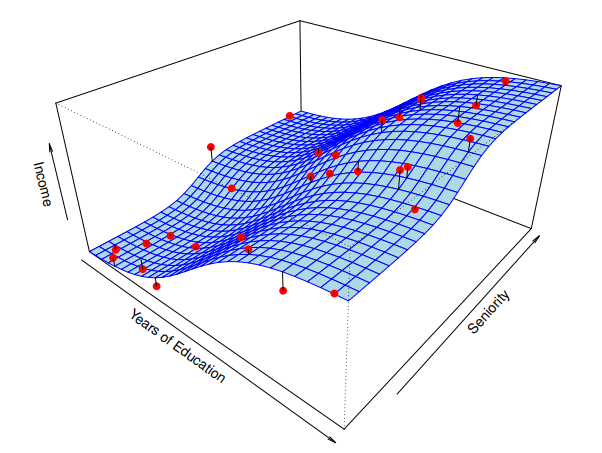
\includegraphics[width=2.94792in,height=\textheight]{images/imagen prediccion.png}

}

\end{figure}

El gráfico muestra los ingresos en función de los años de educación y
antigüedad en el conjunto de datos Renta. La superficie azul representa
la verdadera relación subyacente entre los ingresos y los años de
educación y antigüedad, que se conoce porque los datos son simulados.
Los puntos rojos indican los valores de estas cantidades para 30
individuos.

La exactitud de y depende de dos tipos de error:

\begin{itemize}
\item
  Error reducible: Se refiere a la precisión de las predicciones que
  puede mejorar implementando mejores algoritmos para estimar f(X).
\item
  Error irreducible: Aunque fuera posible obtener la mejor estimación de
  f(X), seguirá existiendo un cierto nivel de incertidumbre ya que
  siempre existen dependencias de la variable objetivo con otras
  variables que no se están considerando o simplemente por procesos
  debidos al azar. Esto es lo que se conoce como error irreducible.
  Siempre proporcionará un límite superior en la precisión de la
  predicción para Y.
\end{itemize}

\textbf{Inferencia}

Para comprender la asociación entre Y y Xp se pueden plantear las
siguientes preguntas:

\begin{enumerate}
\def\labelenumi{\arabic{enumi}.}
\item
  \emph{¿Qué predictores se asocian a la respuesta?}
\item
  \emph{¿Cuál es la relación entre la respuesta y cada predictor?}
\item
  \emph{¿Puede resumirse adecuadamente la relación entre Y y cada
  predictor mediante una ecuación lineal, o la relación es más
  complicada?}
\end{enumerate}

Algunos modelos podrían utilizarse tanto para la predicción como para la
inferencia, dependiendo delobjetivo final. Por ejemplo, los modelos
lineales permiten una inferencia relativamente sencilla y predecible
entre modelos lineales, pero puede que no produzcan predicciones tan
precisas como otros enfoques. Por el contrario, algunos de los enfoques
no lineales pueden brindar información bastante precisas para Y.

\hypertarget{cuxf3mo-estimamos-f}{%
\subsection{¿Cómo estimamos f?}\label{cuxf3mo-estimamos-f}}

\textbf{Métodos paramétricos}: Abarcan un enfoque basado en modelos de
dos pasos:

\begin{enumerate}
\def\labelenumi{\arabic{enumi}.}
\item
  Suposición sobre la forma funcional para el modelo. Ej: f es lineal en
  X.
\item
  Después de seleccionar el modelo se requiere de un procedimiento que
  utilice los datos de entrenamiento para ajustar o entrenar el modelo.
\end{enumerate}

El método más común para ajustar un modelo es el de mínimos cuadrados.

Ejemplo:

\begin{figure}

{\centering 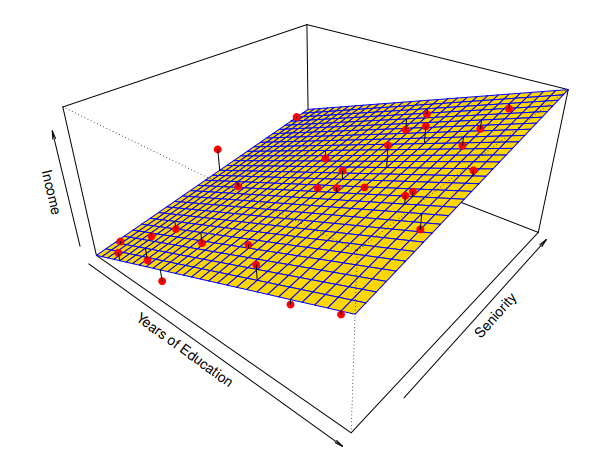
\includegraphics[width=3.92708in,height=\textheight]{images/lineal mod.png}

}

\caption{\emph{Modelo lineal ajustado por mínimos cuadrados a datos de
ingresos. Las observaciones se muestran en rojo, y el plano amarillo
indica el ajuste por mínimos cuadrados a los datos.}}

\end{figure}

El modelo paramétrico reduce el problema para estimar f ya que se
presenta como un conjunto de parámetros en el modelo lineal caso
contario se debería ajustar f a una función arbitraria.

La desventaja de este modelo es que cuando el modelo elegido se aleje
demasiado la estimación será deficiente y para resolver esto se debería
estimar una mayor cantidad de parámetros lo que a su vez podría provocar
un sobreaajuste de datos.

\textbf{Métodos no paramétricos:} Buscan una estimación de f que se
acerque lo más posible a los puntos de datos sin que sea demasiado
aproximada. Se ajustan fácilmente a una gama más amplia de formas
posibles de f.

Una desventaja que presentan es que se necesita un gran número de
observaciones para obtener una estimación precisa de f.

\hypertarget{el-equilibrio-entre-la-precisiuxf3n-de-la-predicciuxf3n-y-la-interpretabilidad-del-modelo}{%
\subsection{El equilibrio entre la precisión de la predicción y la
interpretabilidad del
modelo}\label{el-equilibrio-entre-la-precisiuxf3n-de-la-predicciuxf3n-y-la-interpretabilidad-del-modelo}}

Existen métodos menos flexible o menos restrictivos en el sentido de que
sólo pueden producir una gama relativamente pequeña de formas para
estimar f.

\begin{figure}

{\centering 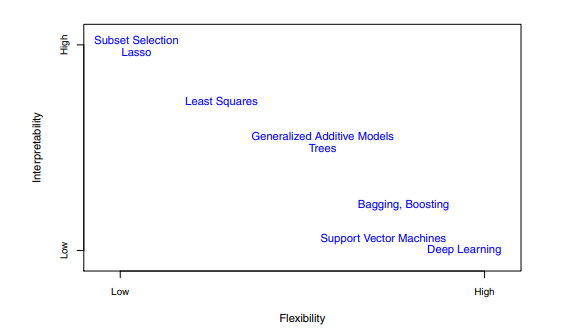
\includegraphics[width=4.86458in,height=\textheight]{images/flexibilidad.png}

}

\caption{\emph{Representación de la relación entre flexibilidad e
interpretabilidad, utilizando diferentes métodos de aprendizaje
estadístico. En general, a medida que aumenta la flexibilidad de un
método, disminuye su interpretabilidad.}}

\end{figure}

\emph{Modelo restrictivo:} Es útil cuando el principal interés es la
inferencia, debido a que es más interpretable.

\emph{Modelos flexibles:} Pueden guiar a estimaciones muy complicadas de
f en las que es difícil comprender cómo se asocia cualquier predictor
con la respuesta.

\begin{itemize}
\item
  lasso: es un enfoque menos flexible y más interpretable que la
  regresión lineal proque en el modelo final la respuesta sólo estará
  relacionada con el modelo final.
\item
  Modelos aditivos generalizados (GAM): Más felxibles que la regresión
  lineal, pero menos interpretables ya que la relación entre cada
  predictor y respuesta se representa mediante una curva.
\item
  Modelos no lineales: bagging, boosting, máquinas de soporte de
  vectores y redes neuronales.
\end{itemize}

\hypertarget{aprendizaje-supervisado-frente-a-aprendizaje-no-supervisado}{%
\subsection{Aprendizaje supervisado frente a aprendizaje no
supervisado}\label{aprendizaje-supervisado-frente-a-aprendizaje-no-supervisado}}

Supervisado: Para cada observación de los predictores hay una respesta
asociada. Permite predecir con exactitud la prespuesta para futuras
predicciones o comprender mejor la relaxción entre predictores y
respuesta.

No supervisado: Se carece de una variable de respuesta que pueda
supervisar el análisis. Es decir no hay una respuesta asociada al
predictor, por lo que no e sposible ajustar a un modelo de regresión
lineal.

\hypertarget{problemas-de-regresiuxf3n-frente-a-problemas-de-clasificaciuxf3n}{%
\subsection{Problemas de regresión frente a problemas de
clasificación}\label{problemas-de-regresiuxf3n-frente-a-problemas-de-clasificaciuxf3n}}

Variables cuantitativas: Toman valores numéricos. Ej: Estatura, edad o
ingresos.

Variables cualitativas: Toman valores en clases o categorías. Ej: Estado
cívil, marcas de productos o diagnósticos.

La regresión logística es un método de clasificación binaria. Es
bastante común seleccionar los métodos de aprendizaje estadístico en
función de si la respuesta es cuantitativa o cualitativa, es decir, se
puede usar la regresión lineal cuando es cuantitativa y la regresión
logística cuando es cualitativa.

\hypertarget{evaluaciuxf3n-de-la-precisiuxf3n-de-los-modelos}{%
\section{Evaluación de la precisión de los
modelos}\label{evaluaciuxf3n-de-la-precisiuxf3n-de-los-modelos}}

En en estadística: ningún método domina a todos los demás en todos los
conjuntos de datos posibles.

\hypertarget{medir-la-calidad-del-ajuste}{%
\subsection{Medir la calidad del
ajuste}\label{medir-la-calidad-del-ajuste}}

Para evaluar el rendimiento de un método de aprendizaje estadístico se
requiere cuantificar hasta qué punto el valor de respuesta predicho para
una observación dada se aproxima al valor de respuesta verdadero para
esa observación.

\emph{Error cuadrático medio (MSE):} será pequeño si las respuestas
predichas están muy cerca de las respuestas verdaderas, y será grande si
para algunas de las observaciones, las respuestas predichas y verdaderas
difieren sustancialmente.

Se calcula utilizando los datos de entrenamiento que se usaron para
jaustar el modelo

\begin{figure}

{\centering 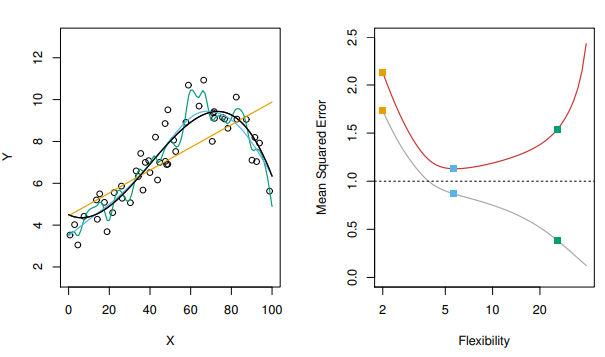
\includegraphics[width=5.01042in,height=\textheight]{images/MSE.png}

}

\caption{\emph{\textbf{Izquierda:} Datos simulados a partir de f,
mostrados en negro. Se muestran tres estimaciones de f: la línea de
regresión lineal (curva naranja) y dos splines de suavizado (curvas azul
y verde). (curvas azul y verde). \textbf{Derecha:} MSE de entrenamiento
(curva gris), MSE de prueba (curva roja roja) y el MSE de prueba mínimo
posible de todos los métodos (línea discontinua). Los cuadrados MSE de
entrenamiento y prueba de los tres ajustes mostrados en el panel
izquierdo.}}

\end{figure}

En la imagen en la parte izquierda se puede ver que a medida que aumenta
el nivel de flexibilidad, las curvas se ajustan mejor a los datos
observados. La curva verde es la más flexible y se ajusta muy bien a los
datos; sin embargo, observamos que se ajusta mal a la f verdadera
(mostrada en negro) porque es demasiado ondulada.

En la parte derecha La curva gris muestra el MSE medio de entrenamiento
en función de la flexibilidad, o más formalmente de los grados de
libertad (flexibilidad de la curva). Los cuadrados naranja, azul y verde
indican los MSE asociados a las curvas.

En este ejemplo, la verdadera f no es lineal, por lo que el ajuste
lineal naranja no es lo suficientemente flexible para estimar bien f.~La
curva verde tiene el MSE de entrenamiento más bajo de los tres métodos,
ya que corresponde al más flexible de ellos. El spline de suavizado
representado por la curva azul se aproxima al óptimo.

En la parte derecha de la figura, a medida que aumenta la flexibilidad
del método de aprendizaje estadístico, observamos un descenso monótono
en el tiempo de entrenamiento. Es decir, a medida que aumenta la
flexibilidad del modelo aumenta, el MSE de entrenamiento disminuirá.

Cuando un método determinado produce un MSE de entrenamiento pequeño
pero un MSE de prueba grande, se dice que se están sobreajustando los
datos.

\hypertarget{la-relaciuxf3n-entre-sesgo-y-varianza}{%
\subsection{La relación entre sesgo y
varianza}\label{la-relaciuxf3n-entre-sesgo-y-varianza}}

Para minimizar el error de prueba esperado se requiere seleccionar un
método de aprendizaje estadístico que consiga simultáneamente baja
varianza y bajo sesgo.

Varianza: Se refire a la cantidad en la que \emph{f} cambiaría si la
estimación se realizara usando un conjunto de datos de enttrenamiento
diferente. Lo ideal es que la estimación de f no varíe demasiado. En
general los métodos estadísticos más flexibles tienen mayor varianza.

Sesgo: Es el error que se introduce al aproximar un problema de la vida
real a un modelo muy simple o sencillo. Es poco probable que un problema
de la vida real tenga una relación lineal tan sencilla, por lo que
realizar una regresión lineal dará lugar a cierto sesgo en la estimación
de f.

La varianza es intrínsecamente una cantidad no negativa, y el sesgo al
cuadrado también es no negativo.

A medida que utilicemos métodos más flexibles, la varianza aumentará y
el sesgo disminuirá.

Un buen rendimiento del conjunto de prueba de un método de aprendizaje
estadístico requiere una varianza baja, así como un equilibrio entre
sesgo y varianza.

\hypertarget{el-entorno-de-clasificaciuxf3n}{%
\subsection{El entorno de
clasificación}\label{el-entorno-de-clasificaciuxf3n}}

Las tasas de error resultantes son de especial interés para la
aplicación del clasificador a observaciones de prueba que no fueron
utilizadas en el entrenamiento. Un buen clasificador es aquel en el que
el error de prueba es mínimo.

\hypertarget{el-clasificador-de-bayes}{%
\subsubsection{El clasificador de
Bayes}\label{el-clasificador-de-bayes}}

Asigna cada observación a la clase más probable dados sus valores
predictores. En un problema de dos clases en el que sólo hay dos
posibles valores de respuesta, el clasificador de Bayes corresponde a la
predicción de la clase uno si Pr(Y = 1\textbar X = x0) \textgreater{}
0,5, y la clase dos en caso contrario.

\begin{figure}

{\centering 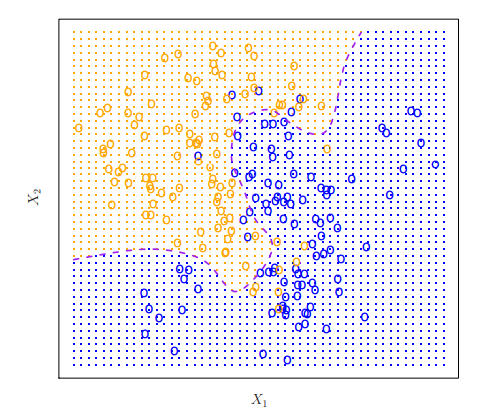
\includegraphics[width=4.28125in,height=\textheight]{images/bayes.png}

}

\caption{\emph{Un conjunto de datos simulados compuesto por 100
observaciones en cada uno de dos grupos, indicados en azul y en naranja.
La línea discontinua morada representa el límite de decisión de Bayes.
La cuadrícula de fondo naranja indica la región en la que una
observación de prueba se asignará a la clase naranja, y la cuadrícula de
fondo azul azul indica la región en la que una observación de prueba se
asignará a la clase azul. a la clase azul.}}

\end{figure}

En la imagen los círculos naranja y azules corresponden a observaciones
de entrenamiento que pertenecen a dos clases diferentes.

Para cada valor de X1 y X2, existe una probabilidad diferente de que la
respuesta sea naranja o azul.

La región sombreada en naranja refleja el conjunto de puntos para los
que Pr(Y = naranja\textbar X) es superior al 50 \%, mientras que la
región sombreada en azul indica el conjunto de puntos cuya probabilidad
es inferior al 50 \%.

La línea discontinua morada representa los puntos en los que la
probabilidad es exactamente del 50 \%. Esto se denomina el
\textbf{límite de decisión de Bayes.}

\hypertarget{k-nearest-neighbors}{%
\subsubsection{K-Nearest Neighbors}\label{k-nearest-neighbors}}

Es utilizado para trabajar con datos reales. Es un algoritmo no
supervisado donde ``K'' representa el número de ``grupos'' (clusters) a
clasificar y el K-neighbor más cercano ``K'' representa el número de
``vecinos'' considerados en los ``n'' grupos del clasificador. En otras
palabras busca en las observaciones más cercanas a la que se está
tratando de predecir y clasifica el punto de interés basado en la
mayoría de datos que le rodean.

\begin{figure}

{\centering 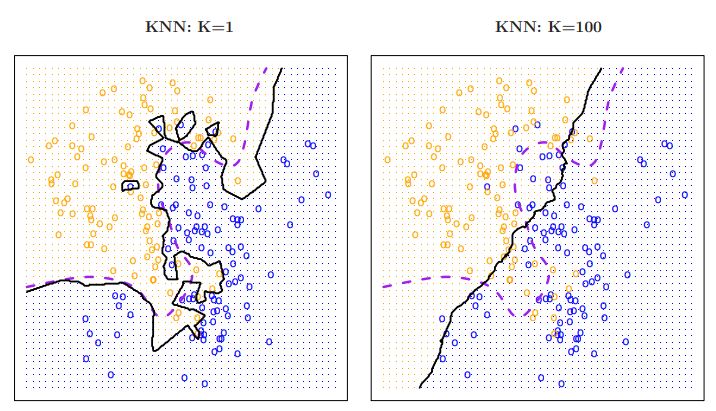
\includegraphics[width=4.64583in,height=\textheight]{images/k-neig.png}

}

\caption{\emph{Comparación de los límites de decisión KNN (curvas negras
obtenidas utilizando K = 1 y K = 100 en los datos de la Figura 2.13. Con
K = 1, el límite de decisión es demasiado flexible, mientras que con K =
100 no es suficientemente flexible. El límite de decisión de Bayes se
muestra como una línea discontinua morada.}}

\end{figure}

La imagen muestra dos ajustes KNN a los datos simulados, utilizando K =
1 y K = 100. Cuando K = 1, el límite de decisión es excesivamente
flexible y encuentra patrones en los datos que no se corresponden con el
límite de decisión de Bayes. Esto corresponde a un clasificador que
tiene un sesgo bajo pero una varianza muy alta. A medida que K aumenta,
el método se vuelve menos flexible y produce una frontera de decisión
cercana a la lineal. Esto corresponde a un clasificador de baja varianza
pero alto sesgo. En este conjunto de datos simulados, ni K = 1 ni K =
100 dan buenas predicciones: tienen tasas de error de prueba de 0,1695 y
0,1925, respectivamente.

\hypertarget{capuxedtulo-3}{%
\section{CAPÍTULO 3}\label{capuxedtulo-3}}

\hypertarget{regresiuxf3n-linear}{%
\section{Regresión linear}\label{regresiuxf3n-linear}}

La regresión lineal, es un enfoque simple pero poderoso para el
aprendizaje supervisado. El capítulo cubre las ideas clave que subyacen
al modelo de regresión lineal, así como el enfoque de mínimos cuadrados
que se usa más comúnmente para ajustar este modelo. También analiza
algunas preguntas importantes que podríamos tratar de abordar al
analizar datos y hacer recomendaciones para planes de marketing basados
en análisis estadísticos. En general, el capítulo sirve como base para
métodos de aprendizaje estadístico más avanzados y proporciona una
descripción general de cómo se puede usar la regresión lineal para
predecir respuestas cuantitativas.

\hypertarget{regresiuxf3n-linear-simple}{%
\subsection{Regresión linear simple}\label{regresiuxf3n-linear-simple}}

La regresión lineal simple es un método estadístico utilizado para
predecir una variable de respuesta cuantitativa basada en una única
variable predictora. Asume que existe una relación aproximadamente
lineal entre el predictor y las variables de respuesta. La relación
lineal se puede expresar matemáticamente como Y ≈ β0 + β1X, donde Y es
la variable de respuesta, X es la variable predictora, β0 y β1 son
coeficientes que representan la intersección y la pendiente de la línea,
respectivamente. El método se usa comúnmente en varios campos, como
marketing, finanzas y ciencias sociales, para analizar datos y hacer
predicciones.

\hypertarget{section}{%
\subsubsection{}\label{section}}

Estimating the Coefficients

Estimar los coeficientes es un paso crucial en la regresión lineal
simple. En la práctica, los coeficientes β0 y β1 son desconocidos, por
lo que antes de que podamos usar el modelo de regresión lineal para
hacer predicciones, debemos usar datos para estimar estos coeficientes.
Se proporciona una discusión detallada sobre cómo estimar estos
coeficientes usando el enfoque de mínimos cuadrados. El enfoque de
mínimos cuadrados implica encontrar los valores de β0 y β1 que minimizan
la suma de los residuos cuadrados entre los valores predichos y reales
de la variable de respuesta.

\begin{figure}

{\centering 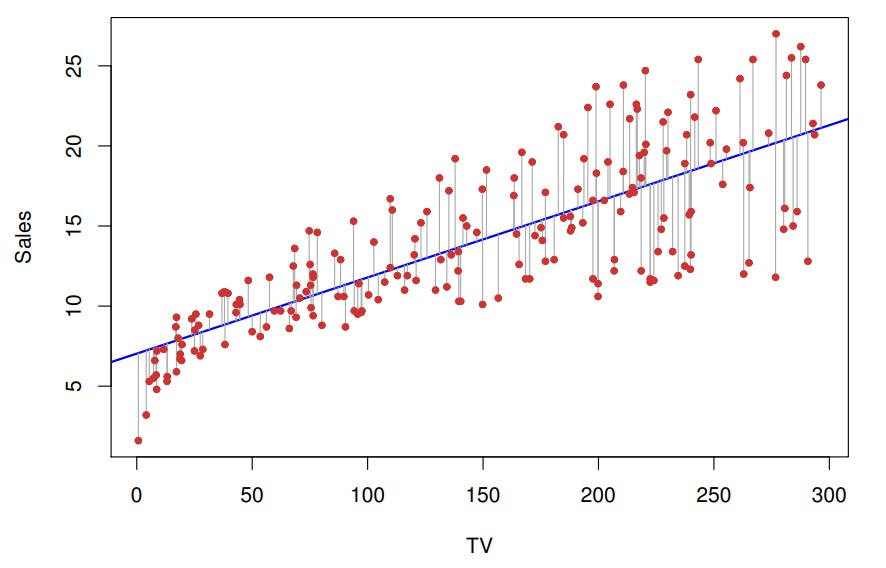
\includegraphics{images/reg.jpg}

}

\caption{FIGURA 1. Para los datos de publicidad, los mínimos cuadrados
se ajustan a la regresión de las ventas en TV se muestra. El ajuste se
obtiene minimizando la suma residual de cuadrícula. Cada segmento de
línea gris representa un residuo. En este caso un ajuste lineal capta la
esencia de la relación, aunque sobrestima la tendencia en la izquierda
de la parcela.}

\end{figure}

\hypertarget{evaluaciuxf3n-de-la-precisiuxf3n-de-las-estimaciones-del-coeficiente}{%
\subsubsection{Evaluación de la precisión de las estimaciones del
coeficiente}\label{evaluaciuxf3n-de-la-precisiuxf3n-de-las-estimaciones-del-coeficiente}}

Es un paso importante en la regresión lineal simple. Una vez que hemos
estimado los coeficientes β0 y β1, es natural querer cuantificar hasta
qué punto estas estimaciones son precisas. presenta una discusión
detallada sobre cómo calcular los errores estándar, las estadísticas t y
los valores p para estas estimaciones de coeficientes. Estas
estadísticas se pueden utilizar para comprobar si existe una relación
lineal significativa entre las variables predictoras y de respuesta, así
como para construir intervalos de confianza para los coeficientes. Se
analiza cómo interpretar estas estadísticas y cómo se pueden usar para
hacer inferencias sobre los parámetros de la población. En general,
evaluar la precisión de las estimaciones de los coeficientes es un paso
esencial en la regresión lineal simple, ya que nos permite determinar si
nuestro modelo es estadísticamente significativo y si nuestras
estimaciones son confiables.

\begin{figure}

{\centering 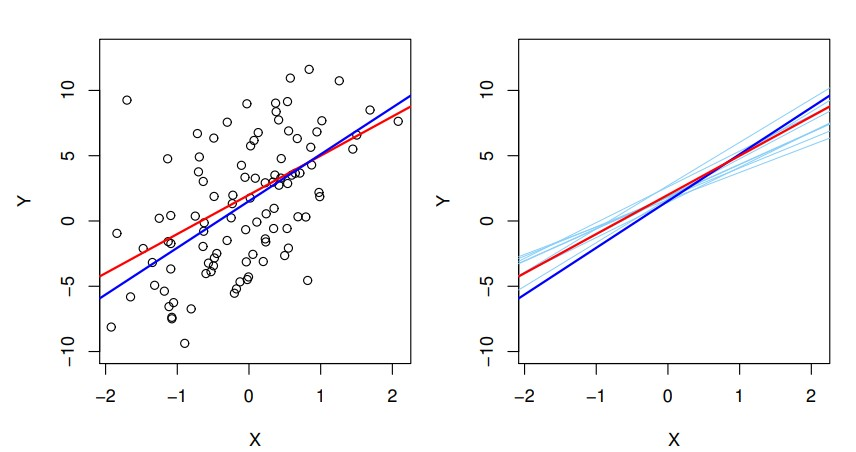
\includegraphics{images/fig4.jpg}

}

\caption{Fig 3. Un conjunto de datos simulado. Izquierda: La línea roja
representa la verdadera relación, f(X)=2+3X, que se conoce como la línea
de regresión de población. El la línea azul es la línea de mínimos
cuadrados; es la estimación de mínimos cuadrados para f(X) basada en los
datos observados, mostrados en negro. Derecha: La línea de regresión de
la población es nuevamente se muestra en rojo, y la línea de mínimos
cuadrados en azul oscuro. En azul claro, diez menos Se muestran líneas
cuadradas, cada una calculada sobre la base de un conjunto aleatorio
separado de observaciones. Cada línea de mínimos cuadrados es diferente,
pero en promedio, los mínimos cuadrados Las líneas están bastante cerca
de la línea de regresión de la población.}

\end{figure}

\begin{figure}

{\centering 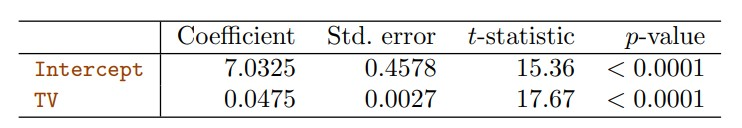
\includegraphics{images/tabl1.jpg}

}

\caption{TABLA 1. Para los datos de Publicidad, coeficientes del modelo
de mínimos cuadrados para la regresión del número de unidades vendidas
sobre el presupuesto de publicidad televisiva. Un aumento de \$1,000 en
el presupuesto de publicidad televisiva se asocia con un aumento en las
ventas de alrededor de 50 unidades. (Recuerde que la variable de ventas
está en miles de unidades, y la La variable TV está en miles de
dólares).}

\end{figure}

\hypertarget{evaluar-la-precisiuxf3n-del-modelo}{%
\subsubsection{Evaluar la precisión del
modelo}\label{evaluar-la-precisiuxf3n-del-modelo}}

Es un paso importante en la regresión lineal simple. Una vez que hemos
rechazado la hipótesis nula a favor de la hipótesis alternativa, es
natural querer cuantificar hasta qué punto el modelo se ajusta a los
datos. La calidad de un ajuste de regresión lineal generalmente se
evalúa utilizando dos cantidades relacionadas: el error estándar
residual (RSE) y la estadística R-cuadrado (R2). El RSE mide la cantidad
promedio que la variable de respuesta se desvía del valor predicho,
mientras que R2 mide qué parte de la variabilidad en la variable de
respuesta puede explicarse por la variable predictora.

\hypertarget{error-estuxe1ndar-residual}{%
\paragraph{Error estándar residual}\label{error-estuxe1ndar-residual}}

El error estándar residual (RSE) es una medida de la cantidad promedio
que la variable de respuesta se desvía del valor predicho en la
regresión lineal simple. Se especifica como calcular RSE usando la
fórmula RSE = sqrt(RSS/(n-2)), donde RSS es la suma residual de los
cuadrados y n es el tamaño de la muestra. El RSE mide la variabilidad de
la variable de respuesta que no está explicada por la variable
predictora, y se puede utilizar para evaluar qué tan bien se ajusta
nuestro modelo a los datos. Un RSE más pequeño indica un mejor ajuste,
mientras que un RSE más grande indica un peor ajuste. Analiza cómo
interpretar RSE y cómo se puede usar junto con otras estadísticas como
R-squared para evaluar la precisión del modelo. Nos permite evaluar qué
tan bien se ajusta nuestro modelo a nuestros datos.

\begin{figure}

{\centering 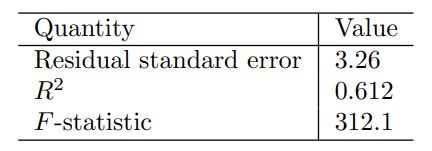
\includegraphics{images/tab2.jpg}

}

\caption{TABLA 2. Para los datos de Publicidad, más información sobre
los mínimos cuadrados modelo para la regresión del número de unidades
vendidas sobre el presupuesto de publicidad televisiva.}

\end{figure}

\hypertarget{regresiuxf3n-lineal-muxfaltiple}{%
\subsection{Regresión lineal
múltiple}\label{regresiuxf3n-lineal-muxfaltiple}}

La regresión lineal múltiple es una extensión de la regresión lineal
simple que nos permite modelar la relación entre una variable de
respuesta y varias variables predictoras. Se muestra cómo realizar una
regresión lineal múltiple utilizando el enfoque de mínimos cuadrados. El
enfoque de mínimos cuadrados implica encontrar los valores de β0, β1,
β2, ..., βp que minimizan la suma de los residuos cuadrados entre los
valores predichos y reales de la variable de respuesta. Muestra como
interpretar estos coeficientes estimados y cómo probar si son
estadísticamente significativos mediante la prueba de hipótesis. Además,
el capítulo cubre temas como la selección de modelos, la
multicolinealidad y los efectos de interacción en la regresión lineal
múltiple. En general, la regresión lineal múltiple es una herramienta
poderosa para modelar relaciones complejas entre variables y se puede
utilizar en una amplia gama de aplicaciones en diversos campos, como la
economía, las finanzas y las ciencias sociales.

\begin{figure}

{\centering 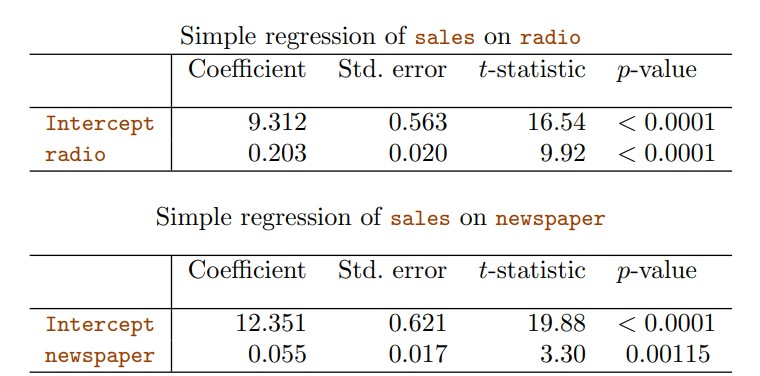
\includegraphics{images/tbl 3.jpg}

}

\caption{Tabla 3. Modelos de regresión lineal más simples para los datos
publicitarios. Coeficientes del modelo de regresión lineal simple para
el número de unidades vendidas en Top: presupuesto de publicidad en
radio y Abajo: presupuesto de publicidad en periódicos. Un aumento de
\$1,000 en el gasto en publicidad por radio está asociado con un aumento
promedio en ventas en alrededor de 203 unidades, mientras que el mismo
aumento en el gasto en publicidad en periódicos está asociado con un
aumento promedio en las ventas de alrededor de 55 unidades. (Nota que la
variable de ventas está en miles de unidades, y la radio y el periódico
las variables están en miles de dólares).}

\end{figure}

\hypertarget{estimaciuxf3n-de-los-coeficientes-de-regresiuxf3n}{%
\subsubsection{Estimación de los coeficientes de
regresión}\label{estimaciuxf3n-de-los-coeficientes-de-regresiuxf3n}}

Se analiza cómo estimar los coeficientes de regresión en Regresión
lineal simple utilizando el enfoque de mínimos cuadrados. El enfoque de
mínimos cuadrados implica encontrar los valores de β0 y β1 que minimizan
la suma de los residuos cuadrados entre los valores predichos y reales
de la variable de respuesta. El capítulo proporciona una discusión
detallada sobre cómo calcular estas estimaciones de coeficientes usando
fórmulas y cómo interpretarlas en el contexto de nuestros datos. Además,
el capítulo cubre temas como errores estándar, estadísticas t y valores
p para estas estimaciones de coeficientes. Estas estadísticas se pueden
utilizar para evaluar la precisión del modelo y construir intervalos de
confianza para los coeficientes. En general, estimar los coeficientes de
regresión es un paso esencial en la regresión lineal simple, ya que nos
permite hacer predicciones basadas en nuestros datos y evaluar qué tan
bien se ajusta nuestro modelo a nuestros datos.

\begin{figure}

{\centering 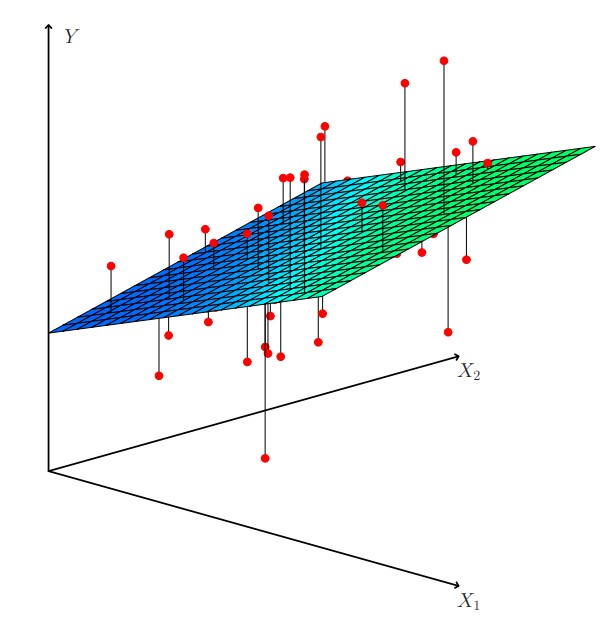
\includegraphics{images/sd.jpg}

}

\caption{FIGURA 4. En un entorno tridimensional, con dos predictores y
una respuesta, la línea de regresión de mínimos cuadrados se convierte
en un plano. El avión es elegido para minimizar la suma de las
distancias verticales al cuadrado entre cada observación (mostrado en
rojo) y el avión.}

\end{figure}

\hypertarget{tabla-4.-para-los-datos-de-publicidad-las-estimaciones-del-coeficiente-de-muxednimos-cuadrados-de-la-regresiuxf3n-lineal-muxfaltiple-del-nuxfamero-de-unidades-vendidas-en-televisiuxf3n-radio-y-periuxf3dicos-presupuestos-publicitarios}{%
\subsubsection{\texorpdfstring{\protect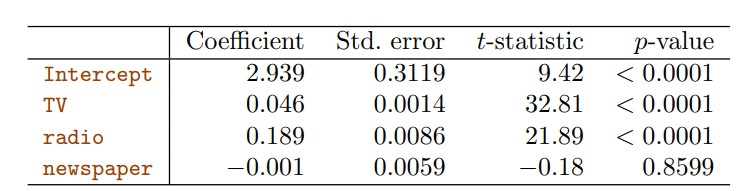
\includegraphics{images/te4.jpg}}{TABLA 4. Para los datos de publicidad, las estimaciones del coeficiente de mínimos cuadrados de la regresión lineal múltiple del número de unidades vendidas en televisión, radio y periódicos presupuestos publicitarios}}\label{tabla-4.-para-los-datos-de-publicidad-las-estimaciones-del-coeficiente-de-muxednimos-cuadrados-de-la-regresiuxf3n-lineal-muxfaltiple-del-nuxfamero-de-unidades-vendidas-en-televisiuxf3n-radio-y-periuxf3dicos-presupuestos-publicitarios}}

\begin{figure}

{\centering 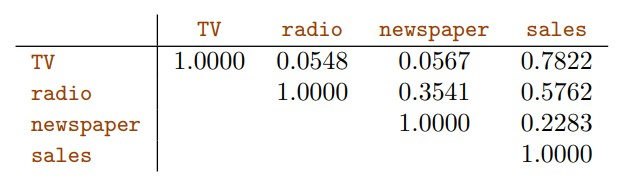
\includegraphics{images/sss.jpg}

}

\caption{Table 5.Matriz de correlación de TV, radio, periódico y ventas
para el Datos publicitarios.}

\end{figure}

\hypertarget{algunas-preguntas-importantes}{%
\subsubsection{Algunas preguntas
importantes}\label{algunas-preguntas-importantes}}

Cuando realizamos una regresión lineal múltiple, por lo general estamos
interesados \hspace{0pt}\hspace{0pt}en respondiendo algunas preguntas
importantes. 1. ¿Al menos uno de los predictores X1, X2,...,Xp es útil
para predecir ¿la respuesta? 2. ¿Todos los predictores ayudan a explicar
Y , o es solo un subconjunto del predictores útil? 3. ¿Qué tan bien se
ajusta el modelo a los datos? 4. Dado un conjunto de valores
predictores, ¿qué valor de respuesta deberíamos predecir? y ¿qué tan
precisa es nuestra predicción? Ahora abordaremos cada una de estas
preguntas por separado.

\hfill\break
Uno: ¿Existe una relación entre la respuesta y los predictores?

Dos: decidir sobre variables importantes\\
Tres: ajuste del modelo Cuatro: predicciones

\hypertarget{otras-consideraciones-en-el-modelo-de-regresiuxf3n}{%
\subsection{Otras consideraciones en el modelo de
regresión}\label{otras-consideraciones-en-el-modelo-de-regresiuxf3n}}

\hypertarget{predictores-cualitativos}{%
\subsubsection{Predictores
cualitativos}\label{predictores-cualitativos}}

En el contexto de la regresión lineal, los predictores cualitativos son
variables que toman valores no numéricos, como categorías o etiquetas.
Por ejemplo, en el conjunto de datos de Crédito que se muestra en la
Figura 6, la variable predictora ``educación'' representa los años de
educación y es una variable cuantitativa, mientras que la variable
predictora ``calificación'' representa la calificación crediticia y es
una variable cualitativa. Cuando se trata de predictores cualitativos en
regresión lineal, necesitamos convertirlos en variables numéricas
mediante un proceso llamado codificación. Un método común para codificar
predictores cualitativos se llama codificación ficticia, donde creamos
variables binarias para representar cada categoría del predictor
cualitativo.

\begin{figure}

{\centering 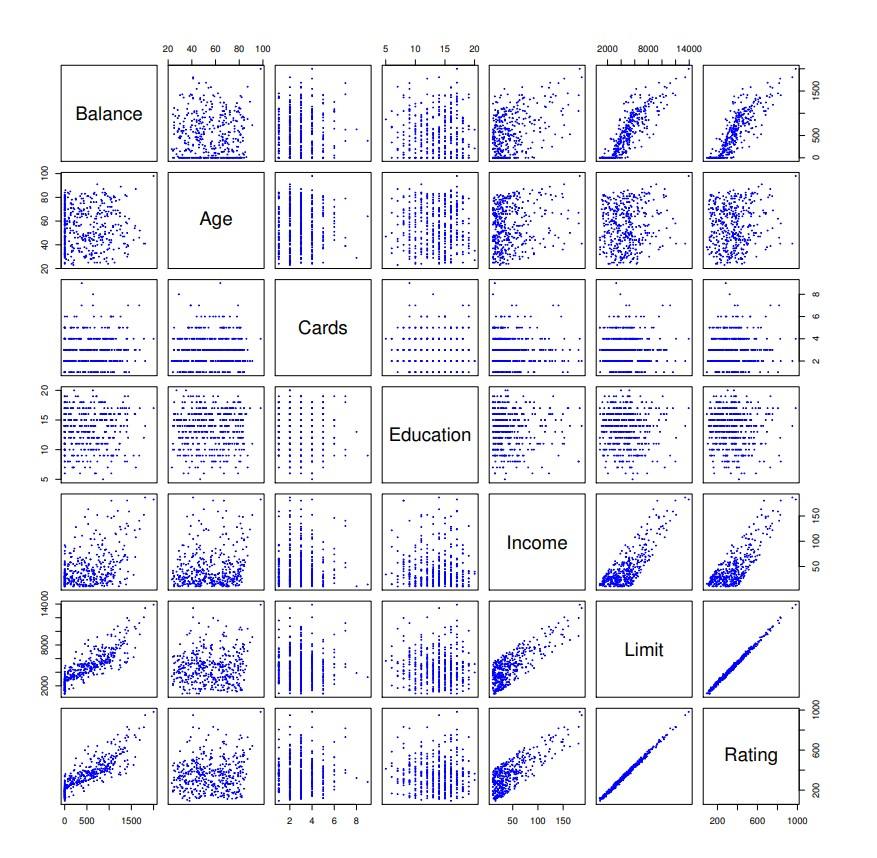
\includegraphics{images/sda.jpg}

}

\caption{FIGURA 6. El conjunto de datos de crédito contiene información
sobre saldo, antigüedad, tarjetas, educación, ingresos, límite y
calificación para una cantidad de clientes potenciales}

\end{figure}

\hypertarget{extensiones-del-modelo-lineal}{%
\subsubsection{Extensiones del modelo
lineal}\label{extensiones-del-modelo-lineal}}

El modelo de regresión lineal estándar hace varias suposiciones
altamente restrictivas que a menudo se violan en la práctica. Dos de los
supuestos más importantes establecen que la relación entre los
predictores y la respuesta es aditiva y lineal. El supuesto de
aditividad significa que la asociación entre un predictor Xj y la
respuesta Y no depende de los valores de los otros predictores. La
suposición de linealidad establece que el cambio en la respuesta Y
asociado con un cambio de una unidad en Xj es constante,
independientemente del valor de Xj.

\begin{figure}

{\centering 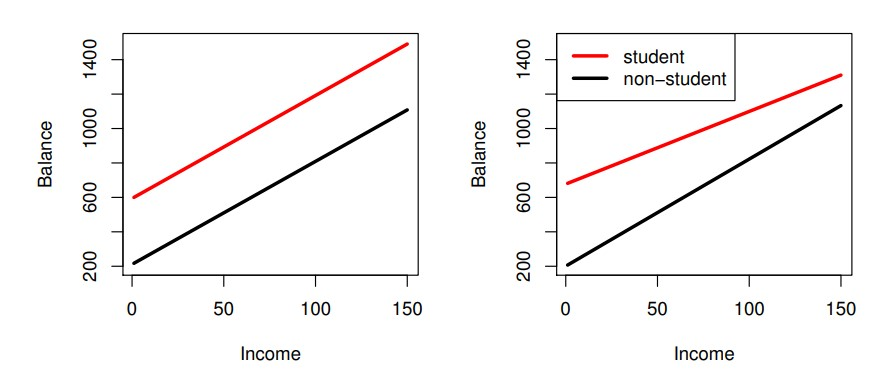
\includegraphics{images/dsads.jpg}

}

\caption{FIGURA 7. Para los datos de crédito, se muestran las líneas de
mínimos cuadrados para la predicción del saldo de ingresos para
estudiantes y no estudiantes. Izquierda: El modelo (3.34) estaba en
forma. No hay interacción entre ingreso y estudiante. Derecha: El el
modelo (3.35) se ajustaba. Existe un término de interacción entre
ingreso y estudiante.}

\end{figure}

Para abordar estas limitaciones, existen varias extensiones del modelo
lineal, como la regresión polinomial, los efectos de interacción y los
modelos lineales generalizados. La regresión polinomial nos permite
modelar relaciones no lineales entre los predictores y la respuesta al
incluir términos de predictores de orden superior en nuestro modelo. Los
efectos de interacción nos permiten modelar cómo dos o más predictores
interactúan entre sí para afectar la variable de respuesta. Los modelos
lineales generalizados amplían la regresión lineal para manejar
variables de respuesta no normales mediante el uso de una función de
enlace para relacionar la media de la variable de respuesta con una
combinación lineal de predictores.

Estas extensiones brindan más flexibilidad en el modelado de problemas
del mundo real donde las relaciones entre predictores y respuestas
pueden no ser estrictamente aditivas o lineales.

\begin{figure}

{\centering 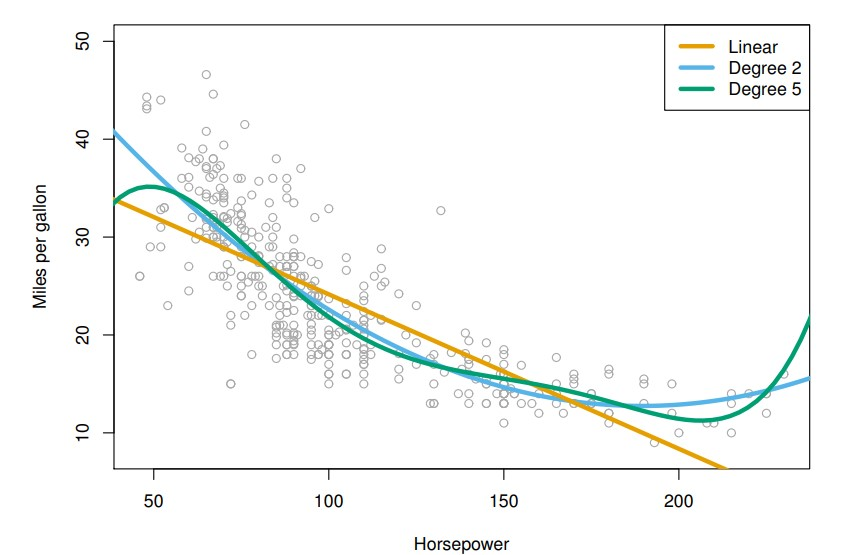
\includegraphics{images/dsad.jpg}

}

\caption{FIGURA 8. El conjunto de datos automático. Para una cantidad de
autos, mpg y caballos de fuerza son mostrado. El ajuste de regresión
lineal se muestra en naranja. El ajuste de regresión lineal para un el
modelo que incluye caballos de fuerza2 se muestra como una curva azul.
La regresión lineal apto para un modelo que incluye todos los polinomios
de caballos de fuerza hasta el quinto grado es se muestra en verde}

\end{figure}

\hypertarget{relaciones-no-lineales}{%
\subsubsection{Relaciones no lineales}\label{relaciones-no-lineales}}

La regresión lineal asume una relación lineal entre la respuesta y los
predictores. Sin embargo, en algunos casos, la verdadera relación entre
la respuesta y los predictores puede no ser lineal. Para dar cabida a
las relaciones no lineales, podemos utilizar la regresión polinomial,
que es una forma sencilla de extender directamente el modelo lineal. La
regresión polinomial nos permite modelar relaciones no lineales entre
los predictores y la respuesta al incluir términos de predictores de
orden superior en nuestro modelo

\hypertarget{problemas-potenciales}{%
\subsubsection{Problemas potenciales}\label{problemas-potenciales}}

\hypertarget{no-linealidad-de-las-relaciones-respuesta-predictor}{%
\paragraph{1. No linealidad de las relaciones
respuesta-predictor}\label{no-linealidad-de-las-relaciones-respuesta-predictor}}

La no linealidad significa que la relación entre la variable de
respuesta y una o más variables predictoras no es lineal, lo que puede
conducir a estimaciones sesgadas o ineficientes de los coeficientes de
regresión. Para abordar la no linealidad, podemos usar la regresión
polinomial, que nos permite modelar relaciones no lineales entre los
predictores y la respuesta al incluir términos de predictores de orden
superior en nuestro modelo.

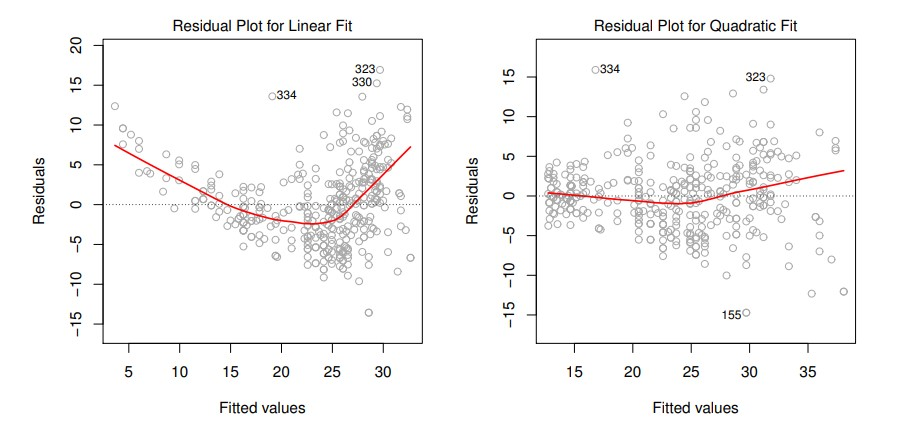
\includegraphics{images/jj.jpg}

\hypertarget{section-1}{%
\paragraph{}\label{section-1}}

\begin{enumerate}
\def\labelenumi{\arabic{enumi}.}
\setcounter{enumi}{1}
\tightlist
\item
  Correlación de términos de error.
\end{enumerate}

Una suposición importante del modelo de regresión lineal es que los
términos de error, ε1, ε2, ..., εn, no están correlacionados. Esto
significa que si los errores no están correlacionados, el hecho de que
εi sea positivo proporciona poca o ninguna información sobre el signo de
εi+1. Los errores estándar que se calculan para los coeficientes de
regresión estimados o los valores ajustados se basan en la suposición de
términos de error no correlacionados. Si de hecho existe una correlación
entre los términos de error, entonces los errores estándar estimados
tenderán a subestimar los errores estándar verdaderos.

\begin{figure}

{\centering 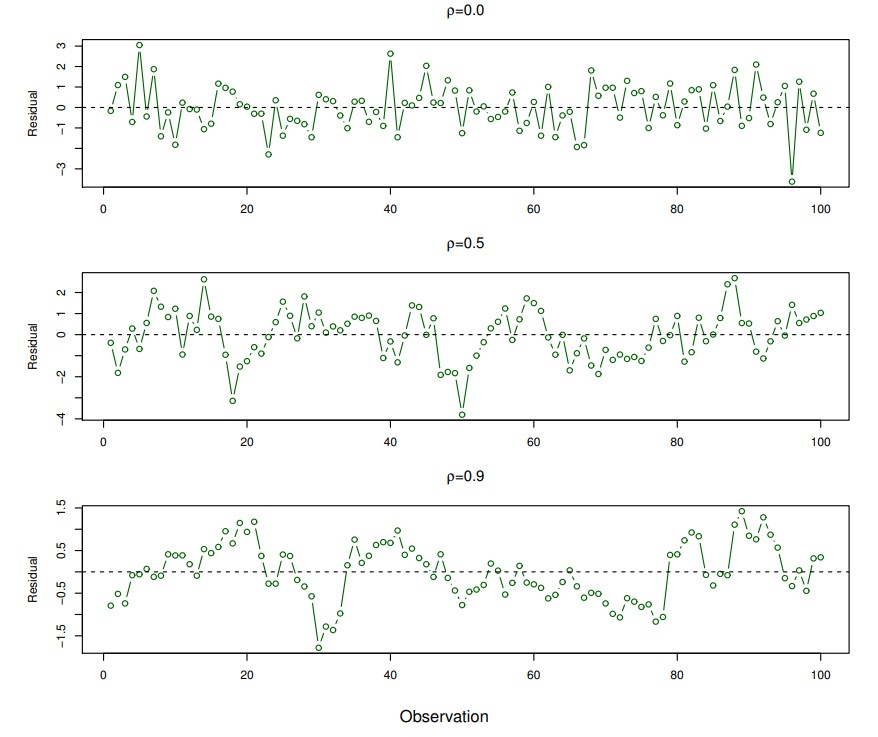
\includegraphics{images/fr.jpg}

}

\caption{FIGURA 10. Gráficas de residuos de conjuntos de datos de series
de tiempo simulados generados con diferentes niveles de correlación ρ
entre términos de error para puntos de tiempo adyacentes.}

\end{figure}

\hypertarget{figura-11.-parcelas-residuales.-en-cada-parcela-la-luxednea-roja-es-un-ajuste-suave-a-la-residuales-destinados-a-facilitar-la-identificaciuxf3n-de-una-tendencia.-las-luxedneas-azules-rastrean-el-cuantiles-externos-de-los-residuales-y-enfatizar-patrones.-izquierda-la-forma-de-embudo-indica-heterocedasticidad.-derecha-la-respuesta-se-ha-transformado-logaruxedtmicamente-y-ahora-no-hay-evidencia-de-heteroscedasticidad.}{%
\paragraph{\texorpdfstring{\protect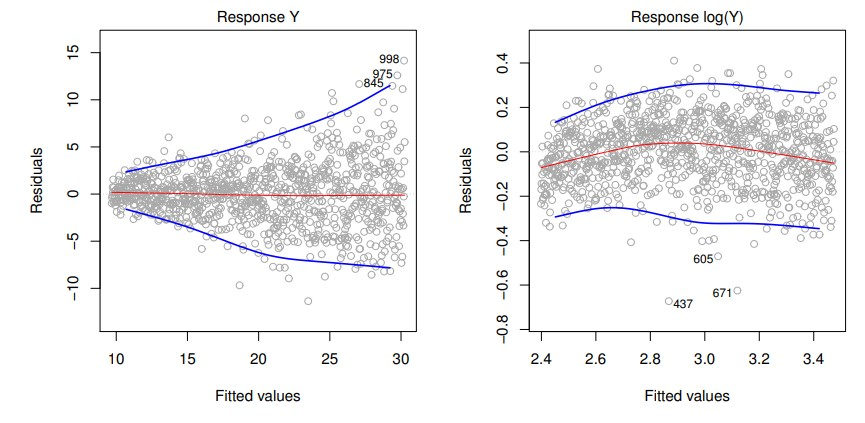
\includegraphics{images/gres.jpg}}{FIGURA 11. Parcelas residuales. En cada parcela, la línea roja es un ajuste suave a la residuales, destinados a facilitar la identificación de una tendencia. Las líneas azules rastrean el cuantiles externos de los residuales y enfatizar patrones. Izquierda: La forma de embudo indica heterocedasticidad. Derecha: la respuesta se ha transformado logarítmicamente y ahora no hay evidencia de heteroscedasticidad.}}\label{figura-11.-parcelas-residuales.-en-cada-parcela-la-luxednea-roja-es-un-ajuste-suave-a-la-residuales-destinados-a-facilitar-la-identificaciuxf3n-de-una-tendencia.-las-luxedneas-azules-rastrean-el-cuantiles-externos-de-los-residuales-y-enfatizar-patrones.-izquierda-la-forma-de-embudo-indica-heterocedasticidad.-derecha-la-respuesta-se-ha-transformado-logaruxedtmicamente-y-ahora-no-hay-evidencia-de-heteroscedasticidad.}}

\begin{enumerate}
\def\labelenumi{\arabic{enumi}.}
\setcounter{enumi}{2}
\tightlist
\item
  Varianza no constante de los términos de error.
\end{enumerate}

Otra suposición importante del modelo de regresión lineal es que los
términos de error tienen una varianza constante, Var(εi)=σ2. Los errores
estándar, los intervalos de confianza y las pruebas de hipótesis
asociadas con el modelo lineal se basan en esta suposición. Si la
varianza de los términos de error no es constante, los errores estándar
estimados estarán sesgados y las pruebas de hipótesis y los intervalos
de confianza no serán válidos. Una forma de abordar la varianza no
constante es usar la regresión de mínimos cuadrados ponderados, que
asigna pesos más grandes a las observaciones con varianzas más pequeñas
y pesos más pequeños a las observaciones con varianzas más grandes.

\hypertarget{figura-12.-izquierda-la-luxednea-de-regresiuxf3n-de-muxednimos-cuadrados-se-muestra-en-rojo-y-la-la-luxednea-de-regresiuxf3n-despuuxe9s-de-eliminar-el-valor-atuxedpico-se-muestra-en-azul.-centro-el-residual-la-trama-identifica-claramente-el-valor-atuxedpico.-derecha-el-valor-atuxedpico-tiene-un-residuo-estudentizado-de-6-tuxedpicamente-esperamos-valores-entre-3-y-3.}{%
\paragraph{\texorpdfstring{\protect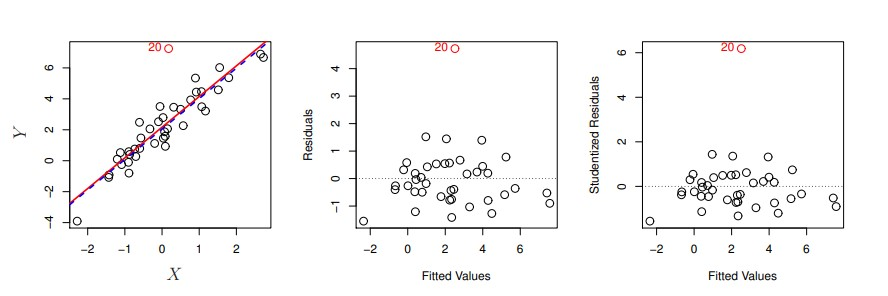
\includegraphics{images/sdas.jpg}}{FIGURA 12. Izquierda: La línea de regresión de mínimos cuadrados se muestra en rojo, y la la línea de regresión después de eliminar el valor atípico se muestra en azul. Centro: El residual la trama identifica claramente el valor atípico. Derecha: El valor atípico tiene un residuo estudentizado de 6; típicamente esperamos valores entre −3 y 3.}}\label{figura-12.-izquierda-la-luxednea-de-regresiuxf3n-de-muxednimos-cuadrados-se-muestra-en-rojo-y-la-la-luxednea-de-regresiuxf3n-despuuxe9s-de-eliminar-el-valor-atuxedpico-se-muestra-en-azul.-centro-el-residual-la-trama-identifica-claramente-el-valor-atuxedpico.-derecha-el-valor-atuxedpico-tiene-un-residuo-estudentizado-de-6-tuxedpicamente-esperamos-valores-entre-3-y-3.}}

\begin{enumerate}
\def\labelenumi{\arabic{enumi}.}
\setcounter{enumi}{3}
\tightlist
\item
  Valores atípicos.
\end{enumerate}

Un valor atípico es un punto para el cual yi está lejos del valor
predicho por el modelo. Los valores atípicos pueden surgir por una
variedad de razones, como el registro incorrecto de una observación
durante la recopilación de datos. Los valores atípicos pueden tener un
gran efecto en los coeficientes de regresión estimados y pueden conducir
a estimaciones sesgadas o ineficientes. Una forma de abordar los valores
atípicos es utilizar métodos de regresión robustos, que son menos
sensibles a los valores atípicos que la regresión ordinaria de mínimos
cuadrados. Otro enfoque es identificar y eliminar los valores atípicos
del conjunto de datos, aunque esto debe hacerse con precaución y solo
después de una cuidadosa consideración de las razones de los valores
atípicos.

\hypertarget{figura-13.-izquierda-la-observaciuxf3n-41-es-un-punto-de-alto-apalancamiento-mientras-que-la-20-no-lo-es.-la-luxednea-roja-es-el-ajuste-a-todos-los-datos-y-la-luxednea-azul-es-el-ajuste-con-la-observaciuxf3n.-41-eliminados.-centro-la-observaciuxf3n-roja-no-es-inusual-en-tuxe9rminos-de-su-valor-x1-o-su-valor-x2-pero-auxfan-queda-fuera-de-la-mayor-parte-de-los-datos-y-por-lo-tanto-tiene-un-alto-aprovechar.-derecha-la-observaciuxf3n-41-tiene-un-alto-apalancamiento-y-un-alto-residual.}{%
\paragraph{\texorpdfstring{\protect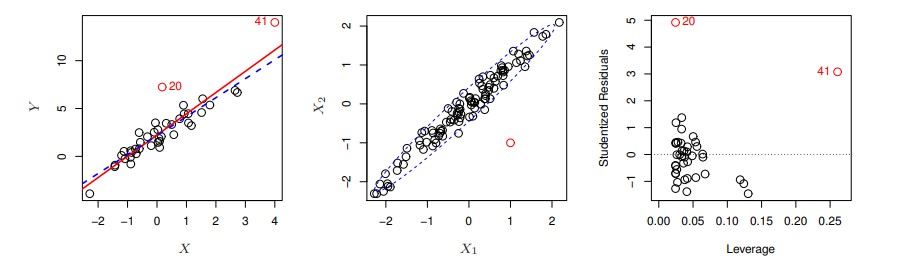
\includegraphics{images/outl.jpg}}{FIGURA 13. Izquierda: la observación 41 es un punto de alto apalancamiento, mientras que la 20 no lo es. La línea roja es el ajuste a todos los datos, y la línea azul es el ajuste con la observación. 41 eliminados. Centro: la observación roja no es inusual en términos de su valor X1 o su valor X2, pero aún queda fuera de la mayor parte de los datos y, por lo tanto, tiene un alto aprovechar. Derecha: la observación 41 tiene un alto apalancamiento y un alto residual.}}\label{figura-13.-izquierda-la-observaciuxf3n-41-es-un-punto-de-alto-apalancamiento-mientras-que-la-20-no-lo-es.-la-luxednea-roja-es-el-ajuste-a-todos-los-datos-y-la-luxednea-azul-es-el-ajuste-con-la-observaciuxf3n.-41-eliminados.-centro-la-observaciuxf3n-roja-no-es-inusual-en-tuxe9rminos-de-su-valor-x1-o-su-valor-x2-pero-auxfan-queda-fuera-de-la-mayor-parte-de-los-datos-y-por-lo-tanto-tiene-un-alto-aprovechar.-derecha-la-observaciuxf3n-41-tiene-un-alto-apalancamiento-y-un-alto-residual.}}

\begin{enumerate}
\def\labelenumi{\arabic{enumi}.}
\setcounter{enumi}{4}
\tightlist
\item
  Puntos de alto apalancamiento.
\end{enumerate}

Los puntos de alto apalancamiento son observaciones con un valor inusual
para xi. Estos puntos pueden tener un gran efecto en los coeficientes de
regresión estimados y pueden conducir a estimaciones sesgadas o
ineficientes. Una forma de identificar puntos de alto apalancamiento es
calcular la estadística de apalancamiento, que mide la influencia de
cada observación en los coeficientes de regresión estimados. Un punto de
alto apalancamiento es aquel para el cual la estadística de
apalancamiento es mucho mayor que el valor promedio de la estadística de
apalancamiento para todas las observaciones. Para abordar los puntos de
alto apalancamiento, podemos usar herramientas de diagnóstico como
gráficos residuales y la distancia de Cook para identificar
observaciones influyentes y potencialmente eliminarlas del conjunto de
datos.

\hypertarget{colinealidad.}{%
\paragraph{6. Colinealidad.}\label{colinealidad.}}

La colinealidad se refiere a la situación en la que dos o más variables
predictoras están estrechamente relacionadas entre sí. La colinealidad
puede dificultar la estimación de los efectos individuales de cada
variable predictora sobre la variable de respuesta y puede conducir a
estimaciones inestables e ineficientes de los coeficientes de regresión.
Una forma de detectar la colinealidad es calcular la matriz de
correlación entre las variables predictoras. Un alto coeficiente de
correlación entre dos variables predictoras indica que pueden ser
colineales. Para abordar la colinealidad, podemos utilizar técnicas como
la regresión de componentes principales o la regresión de crestas, que
pueden ayudar a estabilizar las estimaciones de los coeficientes de
regresión en presencia de predictores colineales.

\begin{figure}

{\centering 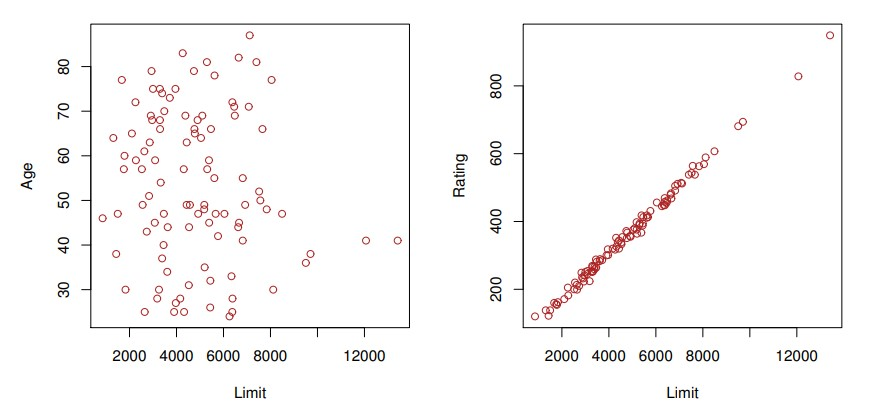
\includegraphics{images/jh.jpg}

}

\caption{FIGURA 14. Diagramas de dispersión de las observaciones del
conjunto de datos Credit. Izquierda: Una gráfica de edad versus límite.
Estas dos variables no son colineales. Derecha: una trama de
calificación versus límite. Hay alta colinealidad.}

\end{figure}

\begin{figure}

{\centering 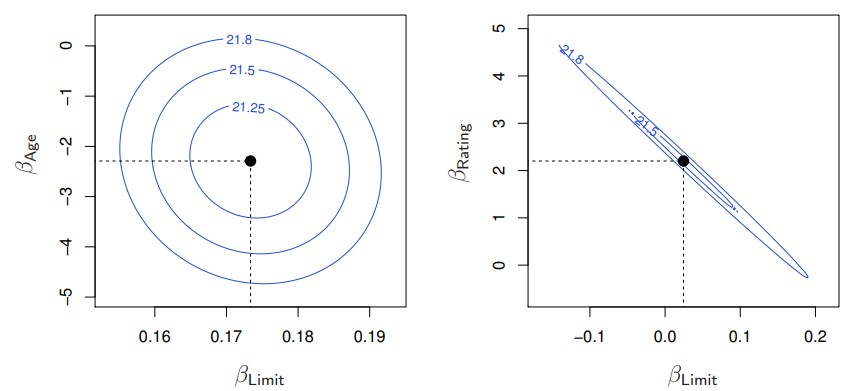
\includegraphics{images/jh1.jpg}

}

\caption{FIGURA 15. Gráficos de contorno para los valores RSS en función
de los parámetros β para varias regresiones que involucran el conjunto
de datos Credit. En cada parcela, el negro los puntos representan los
valores de los coeficientes correspondientes a la RSS mínima. Izquierda:
Un gráfico de contorno de RSS para la regresión del equilibrio sobre la
edad y el límite. El el valor mínimo está bien definido. Derecha: un
gráfico de contorno de RSS para la regresión de equilibrio en
calificación y límite. Debido a la colinealidad, hay muchos pares
(βLimit, βRating) con un valor similar para RSS.}

\end{figure}

\begin{figure}

{\centering 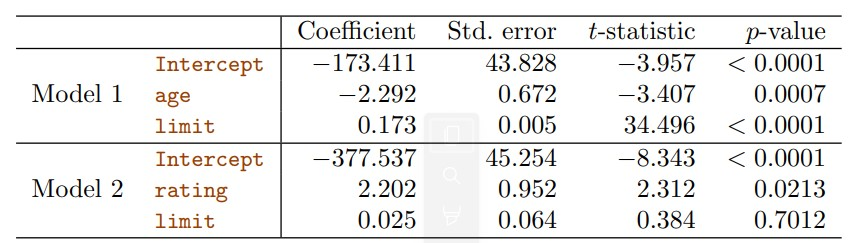
\includegraphics{images/te.jpg}

}

\caption{TABLA 11. Los resultados de dos modelos de regresión múltiple
que implican la Se muestra el conjunto de datos de crédito. El modelo 1
es una regresión de equilibrio sobre edad y límite, y el Modelo 2 una
regresión de equilibrio sobre calificación y límite. El error estándar
de βˆlímite aumenta 12 veces en la segunda regresión, debido a la
colinealidad.}

\end{figure}

\hypertarget{el-plan-de-mercadeo}{%
\subsection{El Plan de Mercadeo}\label{el-plan-de-mercadeo}}

Para responder a las siete preguntas sobre los datos publicitarios que
nos propusimos responder al comienzo de este capítulo, necesitamos
desarrollar un plan de marketing basado en el análisis de los datos. Un
enfoque para desarrollar un plan de marketing es utilizar el análisis de
regresión para modelar la relación entre el presupuesto de publicidad y
las ventas de productos. Podemos usar técnicas como la regresión lineal
múltiple o la regresión polinomial para capturar cualquier relación no
lineal entre estas variables. También podemos utilizar herramientas de
diagnóstico, como gráficos de residuos y pruebas de hipótesis, para
evaluar la bondad de ajuste del modelo e identificar posibles problemas,
como colinealidad o valores atípicos. Con base en los resultados de
nuestro análisis, podemos desarrollar un plan de marketing que se adapte
a las necesidades específicas de la empresa y su público objetivo.

\begin{enumerate}
\def\labelenumi{\arabic{enumi}.}
\tightlist
\item
  ¿Existe una relación entre las ventas y el presupuesto de publicidad?
\item
  ¿Qué tan fuerte es la relación?
\item
  ¿Qué medios están asociados con las ventas?
\item
  ¿Qué tan grande es la asociación entre cada medio y las ventas?
\item
  ¿Con qué precisión podemos predecir las ventas futuras?
\item
  ¿La relación es lineal?
\item
  ¿Existe sinergia entre los medios publicitarios?
\end{enumerate}

\hypertarget{comparaciuxf3n-de-regresiuxf3n-lineal-con-k-vecinos-muxe1s-cercanos}{%
\subsection{Comparación de regresión lineal con K-vecinos más
cercanos}\label{comparaciuxf3n-de-regresiuxf3n-lineal-con-k-vecinos-muxe1s-cercanos}}

La sección presenta una comparación del rendimiento de la regresión
lineal y KNN en conjuntos de datos con relaciones levemente no lineales
y fuertemente no lineales entre las variables predictoras y las
variables de respuesta. Los resultados muestran que KNN puede superar la
regresión lineal en los casos en que la relación entre las variables
predictoras y las variables de respuesta no es lineal. Sin embargo, la
elección del valor de K puede tener un impacto significativo en el
rendimiento de KNN y seleccionar un valor apropiado para K puede ser un
desafío. En general, la elección entre regresión lineal y KNN depende de
las características específicas del conjunto de datos y los objetivos
del análisis.

\begin{figure}

{\centering 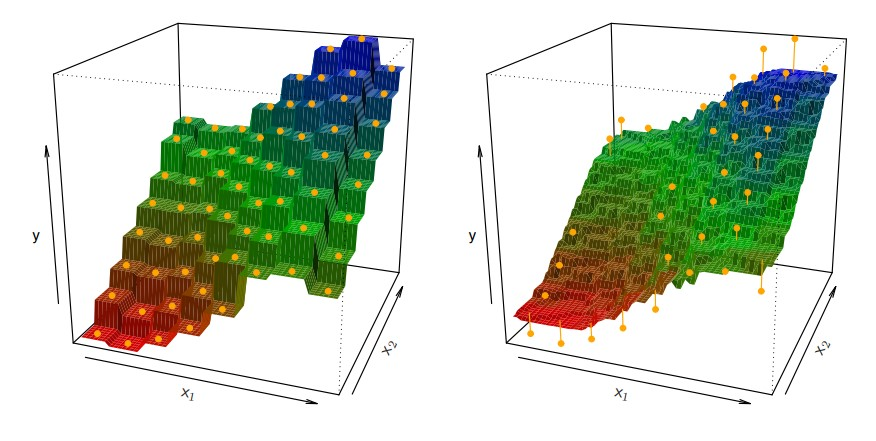
\includegraphics{images/holas.jpg}

}

\caption{FIGURA 16. Gráficas de ˆf(X) usando la regresión KNN en datos
bidimensionales conjunto con 64 observaciones (puntos naranjas).
Izquierda: K = 1 da como resultado un ajuste de función de paso
aproximado. Derecha: K = 9 produce un ajuste mucho más suave}

\end{figure}

\begin{figure}

{\centering 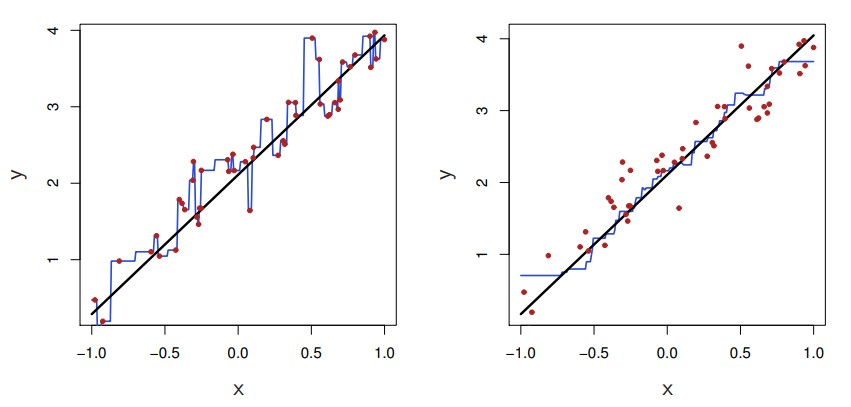
\includegraphics{images/ll.jpg}

}

\caption{FIGURA 17. Gráficas de ˆf(X) usando regresión KNN en datos
unidimensionales conjunto con 50 observaciones. La verdadera relación
viene dada por la línea continua negra. Izquierda: La curva azul
corresponde a K = 1 e interpola (es decir, pasa directamente a través
de) los datos de entrenamiento. Derecha: La curva azul corresponde a K =
9, y representa un ajuste más suave.}

\end{figure}

\begin{figure}

{\centering 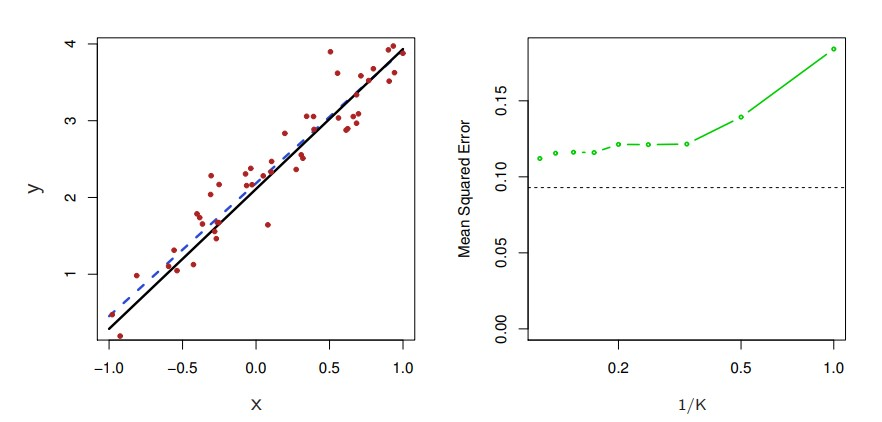
\includegraphics{images/le.jpg}

}

\caption{FIGURA 18. El mismo conjunto de datos que se muestra en la
figura 3.17 se investiga más a fondo. Izquierda: la línea discontinua
azul es el ajuste de mínimos cuadrados a los datos. Como f(X) está en
hecho lineal (mostrado como la línea negra), la línea de regresión de
mínimos cuadrados proporciona una muy buena estimación de f(X). Derecha:
La línea horizontal discontinua representa el conjunto de prueba de
mínimos cuadrados MSE, mientras que la línea continua verde corresponde
al MSE para KNN en función de 1/K (en la escala logarítmica). La
regresión lineal logra un MSE de prueba más bajo que la regresión KNN,
ya que f(X) es de hecho lineal. Para KNN regresión, los mejores
resultados se producen con un valor muy grande de K, correspondiente a
un pequeño valor de 1/K.}

\end{figure}

\begin{figure}

{\centering 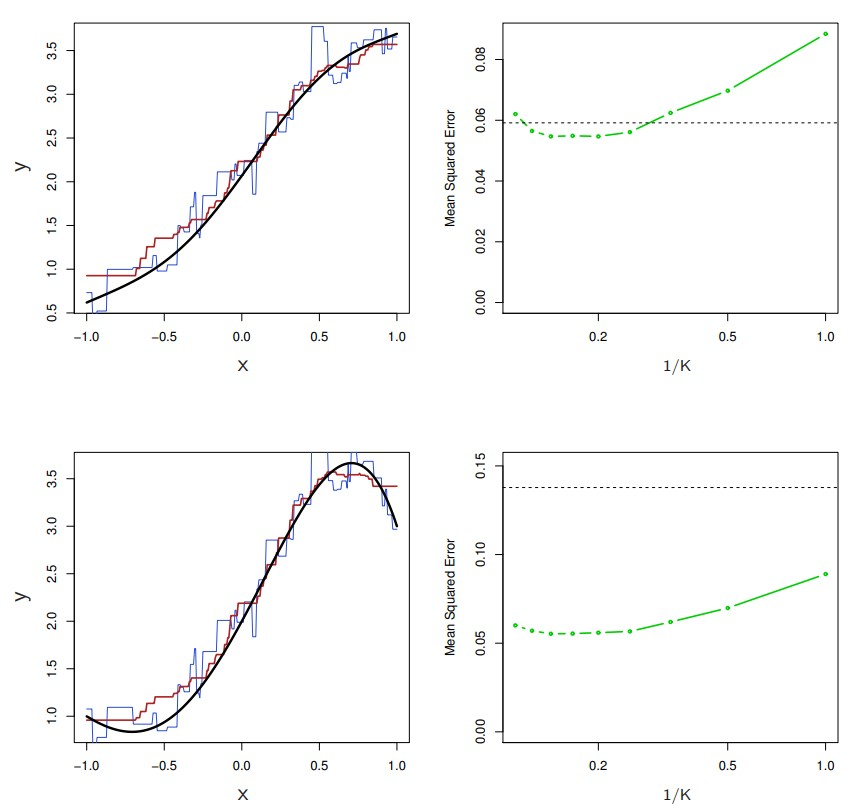
\includegraphics{images/l3.jpg}

}

\caption{FIGURA 19. Arriba a la izquierda: en un entorno con una
relación ligeramente no lineal entre X e Y (línea negra continua), el
KNN encaja con K = 1 (azul) y K = 9 (rojo) se muestran. Arriba a la
derecha: para los datos ligeramente no lineales, el conjunto de prueba
MSE para regresión de mínimos cuadrados (negro horizontal) y KNN con
varios valores de Se muestran 1/K (verde). Inferior izquierda e inferior
derecha: como en el panel superior, pero con una relación fuertemente no
lineal entre X e Y.}

\end{figure}

\begin{figure}

{\centering 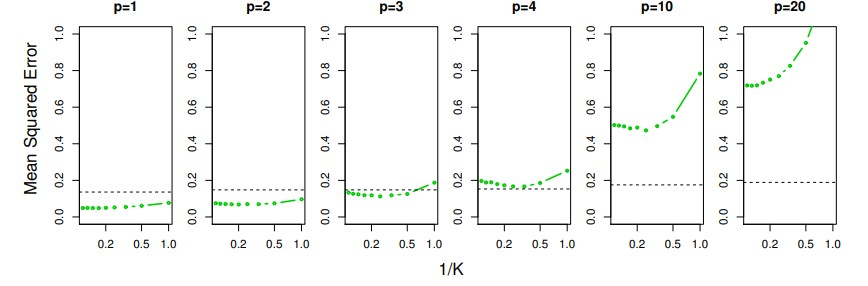
\includegraphics{images/l4.jpg}

}

\caption{FIGURE 20. Test MSE for linear regression (black dashed lines)
and KNN (green curves) as the number of variables p increases. The true
function is non-- linear in the first variable, as in the lower panel in
Figure 3.19, and does not depend on the additional variables. The
performance of linear regression deteriorates slowly in the presence of
these additional noise variables, whereas KNN's performance degrades
much more quickly as p increases.}

\end{figure}

\hypertarget{lab-cap-3---regresiuxf3n-linear}{%
\section{LAB: CAP 3 - Regresión
linear}\label{lab-cap-3---regresiuxf3n-linear}}

Librerías a usar:

MASS: colección de conjunto de datos y funciones.

ISLR2: Conjunto de datos asociados al libro de estudio.

\begin{Shaded}
\begin{Highlighting}[]
\FunctionTok{library}\NormalTok{ (MASS)}
\FunctionTok{library}\NormalTok{ (ISLR2)}
\end{Highlighting}
\end{Shaded}

\begin{verbatim}

Attaching package: 'ISLR2'
\end{verbatim}

\begin{verbatim}
The following object is masked from 'package:MASS':

    Boston
\end{verbatim}

\hypertarget{regresiuxf3n-linear-simple-1}{%
\subsection{Regresión linear
simple}\label{regresiuxf3n-linear-simple-1}}

La biblioteca ISLR2 contiene el conjunto de datos de Boston, que
registra el medv (valor medio de la vivienda) de 506 secciones censales
de Boston. Intentaremos predecir medv utilizando 12 predictores como rm
(número medio de habitaciones por casa) edad (edad media de las casas) y
lstat (porcentaje de hogares con un estatus socioeconómico bajo).

\begin{Shaded}
\begin{Highlighting}[]
\FunctionTok{head}\NormalTok{(Boston)}
\end{Highlighting}
\end{Shaded}

\begin{verbatim}
     crim zn indus chas   nox    rm  age    dis rad tax ptratio lstat medv
1 0.00632 18  2.31    0 0.538 6.575 65.2 4.0900   1 296    15.3  4.98 24.0
2 0.02731  0  7.07    0 0.469 6.421 78.9 4.9671   2 242    17.8  9.14 21.6
3 0.02729  0  7.07    0 0.469 7.185 61.1 4.9671   2 242    17.8  4.03 34.7
4 0.03237  0  2.18    0 0.458 6.998 45.8 6.0622   3 222    18.7  2.94 33.4
5 0.06905  0  2.18    0 0.458 7.147 54.2 6.0622   3 222    18.7  5.33 36.2
6 0.02985  0  2.18    0 0.458 6.430 58.7 6.0622   3 222    18.7  5.21 28.7
\end{verbatim}

\begin{itemize}
\item
  \textbf{?Boston:} Para obtener información sobre el conjunto de datos.
\item
  \textbf{lm():} Para ajustar un modelo de regresión lineal simple.
\item
  \textbf{Predictor:} Istat
\item
  \textbf{Respuesta:} medv
\end{itemize}

La sintaxis básica es lm(y ∼ x, datos), donde y es la respuesta, x es el
predictor y datos es el conjunto de datos en el que se mantienen estas
dos variables.

\begin{Shaded}
\begin{Highlighting}[]
\FunctionTok{attach}\NormalTok{(Boston)}
\NormalTok{lm.fit}\OtherTok{\textless{}{-}}\FunctionTok{lm}\NormalTok{(medv}\SpecialCharTok{\textasciitilde{}}\NormalTok{lstat,}\AttributeTok{data =}\NormalTok{ Boston)}
\NormalTok{lm.fit}\OtherTok{\textless{}{-}}\FunctionTok{lm}\NormalTok{(medv}\SpecialCharTok{\textasciitilde{}}\NormalTok{lstat)}
\end{Highlighting}
\end{Shaded}

Si escribimos lm.fit, aparecerá información básica sobre el modelo.

Para obtener información más detallada, utilice summary(lm.fit). Se
obtienen los valores p y los errores estándar de los coeficientes, así
como el estadístico R2 y el estadístico F del modelo.

\begin{Shaded}
\begin{Highlighting}[]
\NormalTok{lm.fit}
\end{Highlighting}
\end{Shaded}

\begin{verbatim}

Call:
lm(formula = medv ~ lstat)

Coefficients:
(Intercept)        lstat  
      34.55        -0.95  
\end{verbatim}

\begin{Shaded}
\begin{Highlighting}[]
\FunctionTok{summary}\NormalTok{(lm.fit)}
\end{Highlighting}
\end{Shaded}

\begin{verbatim}

Call:
lm(formula = medv ~ lstat)

Residuals:
    Min      1Q  Median      3Q     Max 
-15.168  -3.990  -1.318   2.034  24.500 

Coefficients:
            Estimate Std. Error t value Pr(>|t|)    
(Intercept) 34.55384    0.56263   61.41   <2e-16 ***
lstat       -0.95005    0.03873  -24.53   <2e-16 ***
---
Signif. codes:  0 '***' 0.001 '**' 0.01 '*' 0.05 '.' 0.1 ' ' 1

Residual standard error: 6.216 on 504 degrees of freedom
Multiple R-squared:  0.5441,    Adjusted R-squared:  0.5432 
F-statistic: 601.6 on 1 and 504 DF,  p-value: < 2.2e-16
\end{verbatim}

Podemos utilizar la función names() para averiguar qué otras piezas
nombres de información se almacenan en lm.fit.

Es más seguro utilizar las funciones extractoras como coef() para
acceder a ellas.

\begin{Shaded}
\begin{Highlighting}[]
\FunctionTok{names}\NormalTok{(lm.fit)}
\end{Highlighting}
\end{Shaded}

\begin{verbatim}
 [1] "coefficients"  "residuals"     "effects"       "rank"         
 [5] "fitted.values" "assign"        "qr"            "df.residual"  
 [9] "xlevels"       "call"          "terms"         "model"        
\end{verbatim}

\begin{Shaded}
\begin{Highlighting}[]
\FunctionTok{coef}\NormalTok{(lm.fit)}
\end{Highlighting}
\end{Shaded}

\begin{verbatim}
(Intercept)       lstat 
 34.5538409  -0.9500494 
\end{verbatim}

confint(): Para obtener un intervalo de confianza para las estimaciones
de los coeficientes.

\begin{Shaded}
\begin{Highlighting}[]
\FunctionTok{confint}\NormalTok{(lm.fit)}
\end{Highlighting}
\end{Shaded}

\begin{verbatim}
                2.5 %     97.5 %
(Intercept) 33.448457 35.6592247
lstat       -1.026148 -0.8739505
\end{verbatim}

predict(): Usada para producir intervalos de confianza para la
predicción de medv para un valor dado de lstat.

\begin{Shaded}
\begin{Highlighting}[]
\FunctionTok{predict}\NormalTok{(lm.fit,}\FunctionTok{data.frame}\NormalTok{(}\AttributeTok{lstat=}\NormalTok{(}\FunctionTok{c}\NormalTok{(}\DecValTok{5}\NormalTok{,}\DecValTok{10}\NormalTok{,}\DecValTok{15}\NormalTok{))),}\AttributeTok{interval =} \StringTok{"confidence"}\NormalTok{)}
\end{Highlighting}
\end{Shaded}

\begin{verbatim}
       fit      lwr      upr
1 29.80359 29.00741 30.59978
2 25.05335 24.47413 25.63256
3 20.30310 19.73159 20.87461
\end{verbatim}

\begin{Shaded}
\begin{Highlighting}[]
\FunctionTok{predict}\NormalTok{(lm.fit,}\FunctionTok{data.frame}\NormalTok{(}\AttributeTok{lstat=}\NormalTok{(}\FunctionTok{c}\NormalTok{(}\DecValTok{5}\NormalTok{,}\DecValTok{10}\NormalTok{,}\DecValTok{15}\NormalTok{))),}\AttributeTok{interval =} \StringTok{"prediction"}\NormalTok{)}
\end{Highlighting}
\end{Shaded}

\begin{verbatim}
       fit       lwr      upr
1 29.80359 17.565675 42.04151
2 25.05335 12.827626 37.27907
3 20.30310  8.077742 32.52846
\end{verbatim}

Por ejemplo, el intervalo de confianza del 95 \% asociado a un valor
lstat de 10 es (24.47, 25.63), y el intervalo de predicción del 95 \% es
(12.828, 37.28). Como era de esperar, los intervalos de confianza y
predicción se centran en el mismo punto (un valor predicho de 10). En el
mismo punto (un valor predicho de 25,05 para medv cuando lstat es igual
a 10), pero estos últimos son mucho más amplios.

Ahora trazaremos medv y lstat junto con la línea de regresión por
mínimos cuadrados utilizando las funciones plot() y abline().
\textbf{abline():} se puede usar para agregar líneas verticales,
horizontales o de regresión a un gráfico.

\begin{Shaded}
\begin{Highlighting}[]
\FunctionTok{plot}\NormalTok{(lstat,medv)}
\FunctionTok{abline}\NormalTok{(lm.fit)}
\end{Highlighting}
\end{Shaded}

\begin{figure}[H]

{\centering 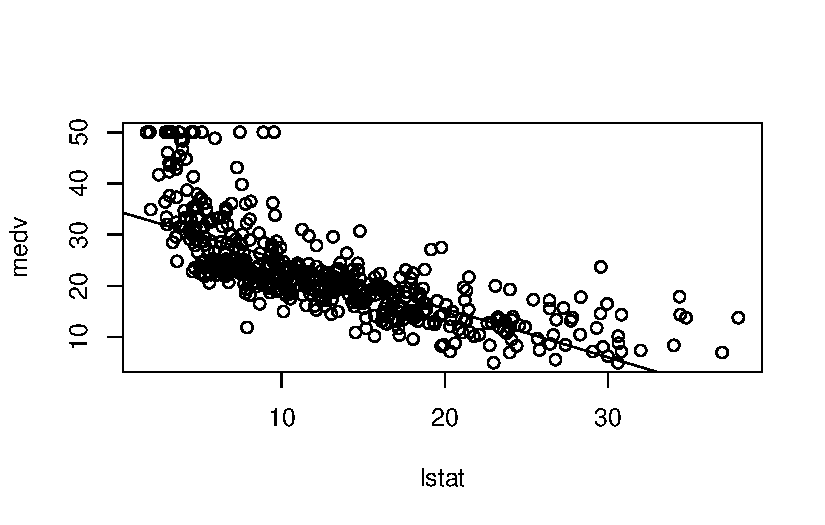
\includegraphics{Resumen-2---3_files/figure-pdf/unnamed-chunk-8-1.pdf}

}

\end{figure}

Se puede observar indicios de no linealidad en la relación entre lstat y
medv.

En la función abline() para dibujar una recta con intersección en a y
pendiente b, se escribe \textbf{abline(a,b)}. Unos ajustes adicionales
para trazar líneas y puntos son:

\begin{itemize}
\item
  lwd: Para la anchura de la línea de regresión.
\item
  pch: Para crear diferentes símbolos de trazado.
\end{itemize}

\begin{Shaded}
\begin{Highlighting}[]
\FunctionTok{plot}\NormalTok{(lstat,medv)}
\FunctionTok{abline}\NormalTok{ (lm.fit , }\AttributeTok{lwd =} \DecValTok{3}\NormalTok{)}
\FunctionTok{abline}\NormalTok{ (lm.fit , }\AttributeTok{lwd =} \DecValTok{3}\NormalTok{, }\AttributeTok{col =} \StringTok{" red "}\NormalTok{)}
\end{Highlighting}
\end{Shaded}

\begin{figure}[H]

{\centering 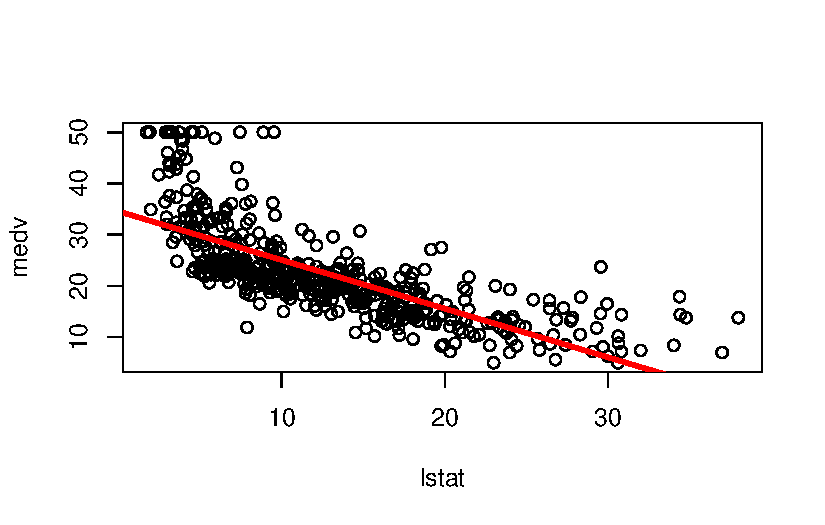
\includegraphics{Resumen-2---3_files/figure-pdf/unnamed-chunk-9-1.pdf}

}

\end{figure}

\begin{Shaded}
\begin{Highlighting}[]
\FunctionTok{plot}\NormalTok{ (lstat , medv , }\AttributeTok{col =} \StringTok{" red "}\NormalTok{)}
\end{Highlighting}
\end{Shaded}

\begin{figure}[H]

{\centering 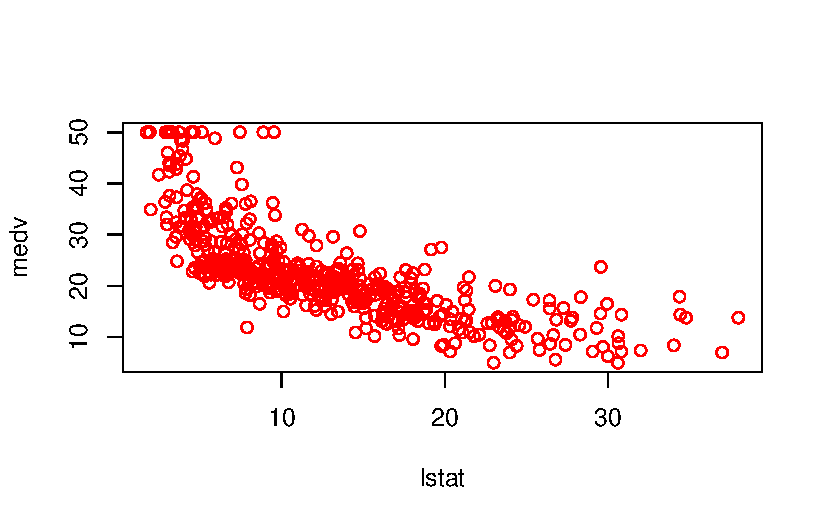
\includegraphics{Resumen-2---3_files/figure-pdf/unnamed-chunk-9-2.pdf}

}

\end{figure}

\begin{Shaded}
\begin{Highlighting}[]
\FunctionTok{plot}\NormalTok{ (lstat , medv , }\AttributeTok{pch =} \DecValTok{20}\NormalTok{)}
\end{Highlighting}
\end{Shaded}

\begin{figure}[H]

{\centering 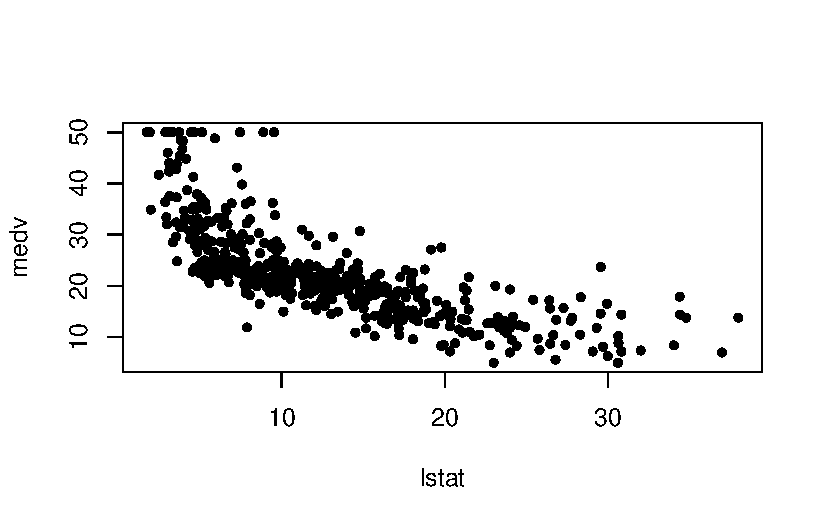
\includegraphics{Resumen-2---3_files/figure-pdf/unnamed-chunk-9-3.pdf}

}

\end{figure}

\begin{Shaded}
\begin{Highlighting}[]
\FunctionTok{plot}\NormalTok{ (lstat , medv , }\AttributeTok{pch =} \StringTok{"+"}\NormalTok{)}
\end{Highlighting}
\end{Shaded}

\begin{figure}[H]

{\centering 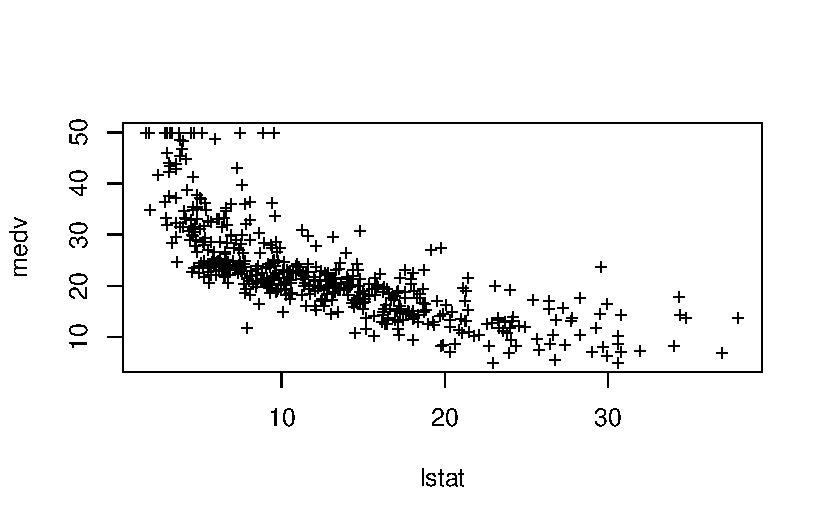
\includegraphics{Resumen-2---3_files/figure-pdf/unnamed-chunk-9-4.pdf}

}

\end{figure}

\begin{Shaded}
\begin{Highlighting}[]
\FunctionTok{plot}\NormalTok{ (}\DecValTok{1}\SpecialCharTok{:}\DecValTok{20}\NormalTok{, }\DecValTok{1}\SpecialCharTok{:}\DecValTok{20}\NormalTok{, }\AttributeTok{pch =} \DecValTok{1}\SpecialCharTok{:}\DecValTok{20}\NormalTok{)}
\end{Highlighting}
\end{Shaded}

\begin{figure}[H]

{\centering 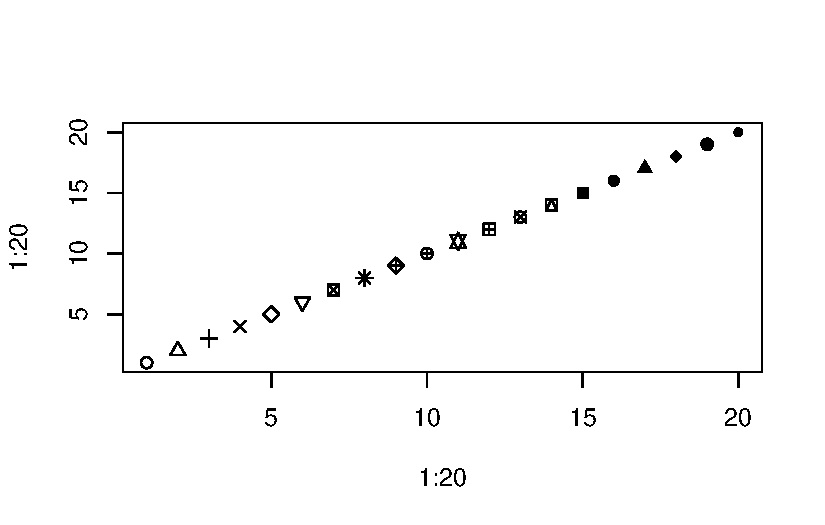
\includegraphics{Resumen-2---3_files/figure-pdf/unnamed-chunk-9-5.pdf}

}

\end{figure}

par() y mfrow(): Indicaan a R que divida la pantalla de vizualización en
paneles separados para poder visualizar gráficos simultaneamente.

\begin{Shaded}
\begin{Highlighting}[]
\FunctionTok{plot}\NormalTok{(lm.fit)}
\end{Highlighting}
\end{Shaded}

\begin{figure}[H]

{\centering 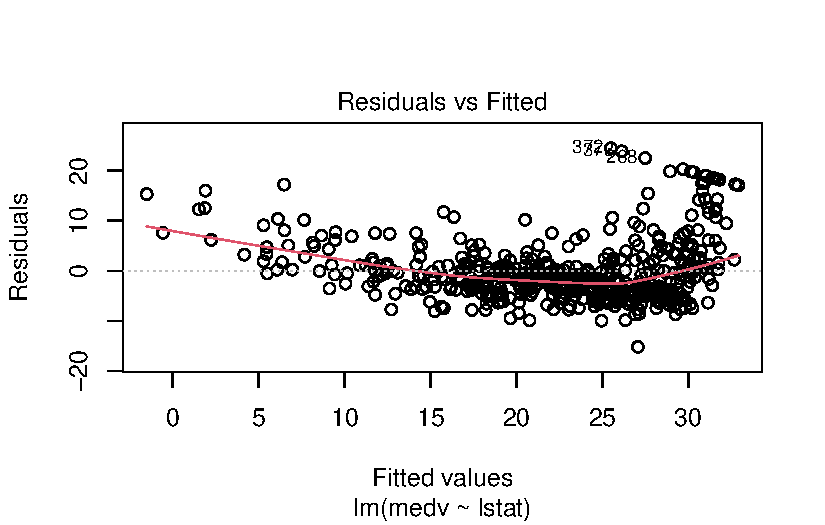
\includegraphics{Resumen-2---3_files/figure-pdf/unnamed-chunk-10-1.pdf}

}

\end{figure}

\begin{figure}[H]

{\centering 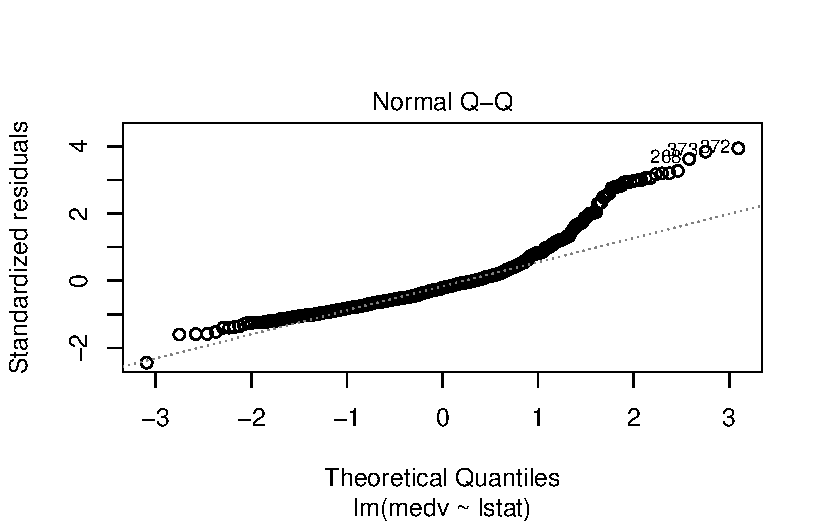
\includegraphics{Resumen-2---3_files/figure-pdf/unnamed-chunk-10-2.pdf}

}

\end{figure}

\begin{figure}[H]

{\centering 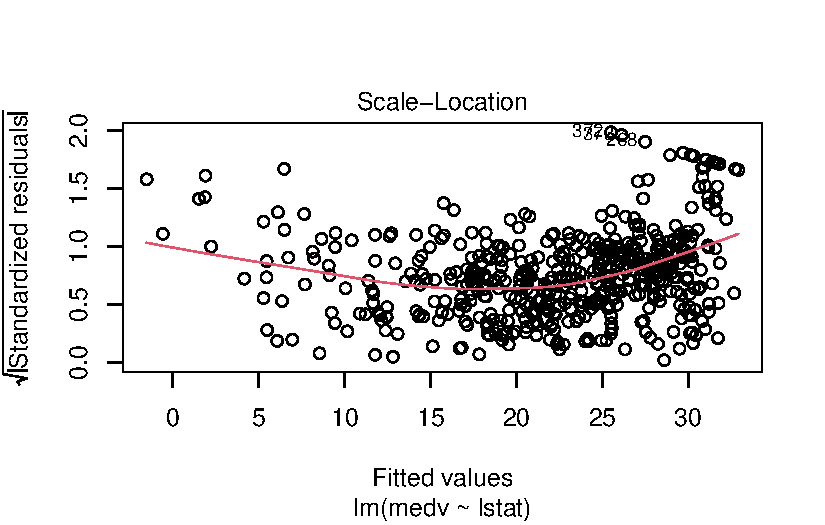
\includegraphics{Resumen-2---3_files/figure-pdf/unnamed-chunk-10-3.pdf}

}

\end{figure}

\begin{figure}[H]

{\centering 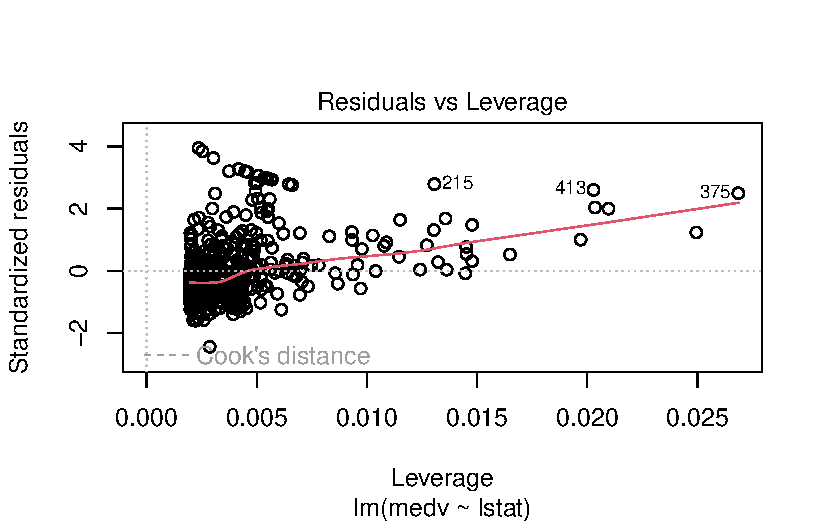
\includegraphics{Resumen-2---3_files/figure-pdf/unnamed-chunk-10-4.pdf}

}

\end{figure}

\begin{Shaded}
\begin{Highlighting}[]
\FunctionTok{par}\NormalTok{(}\AttributeTok{mfrow=}\FunctionTok{c}\NormalTok{(}\DecValTok{2}\NormalTok{,}\DecValTok{2}\NormalTok{))}
\end{Highlighting}
\end{Shaded}

residuals (): Para calcular los residuos de un ajuste de regresión
lineal.

rstudent(): Devuelve los residuales estudiados y se puede usar para
representar gráficamente los residuos frente a los valores ajustados

\begin{Shaded}
\begin{Highlighting}[]
\FunctionTok{plot}\NormalTok{ ( }\FunctionTok{predict}\NormalTok{ (lm.fit), }\FunctionTok{residuals}\NormalTok{ (lm.fit))}
\end{Highlighting}
\end{Shaded}

\begin{figure}[H]

{\centering 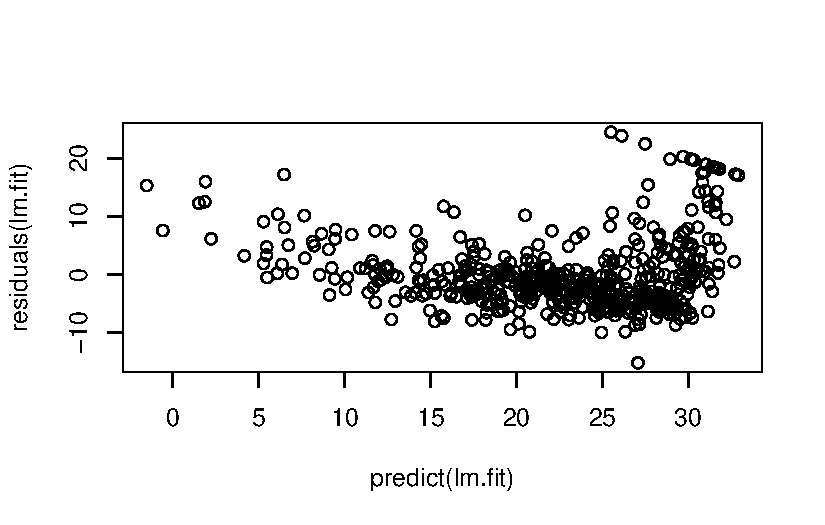
\includegraphics{Resumen-2---3_files/figure-pdf/unnamed-chunk-11-1.pdf}

}

\end{figure}

\begin{Shaded}
\begin{Highlighting}[]
\FunctionTok{plot}\NormalTok{ ( }\FunctionTok{predict}\NormalTok{ (lm.fit), }\FunctionTok{rstudent}\NormalTok{ (lm.fit))}
\end{Highlighting}
\end{Shaded}

\begin{figure}[H]

{\centering 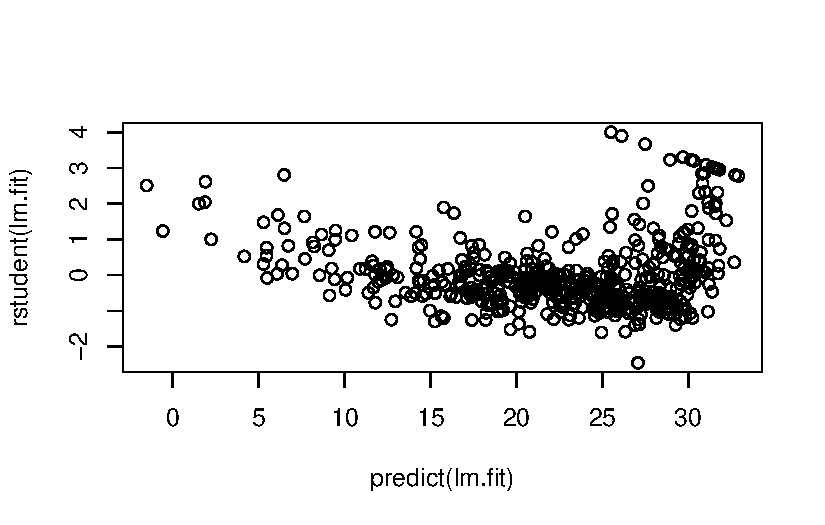
\includegraphics{Resumen-2---3_files/figure-pdf/unnamed-chunk-11-2.pdf}

}

\end{figure}

hatvalues(): Sirve para calcular los estadísticos utilizando cualquier
número de predictores.

which max: identifica el índice del elemento mayor de un vector. En este
caso dice que la observación tiene el mayor estadístico de
apalancamiento (375).

\begin{Shaded}
\begin{Highlighting}[]
\FunctionTok{plot}\NormalTok{ ( }\FunctionTok{hatvalues}\NormalTok{ (lm.fit))}
\end{Highlighting}
\end{Shaded}

\begin{figure}[H]

{\centering 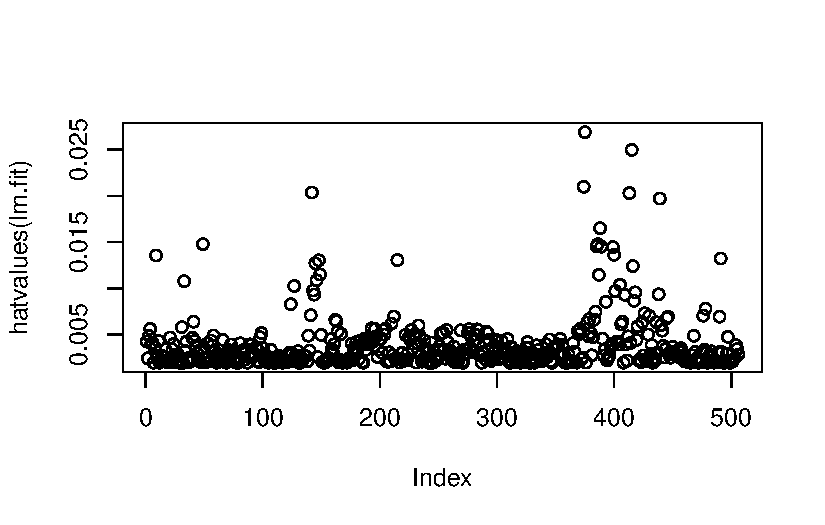
\includegraphics{Resumen-2---3_files/figure-pdf/unnamed-chunk-12-1.pdf}

}

\end{figure}

\begin{Shaded}
\begin{Highlighting}[]
\FunctionTok{which.max}\NormalTok{( }\FunctionTok{hatvalues}\NormalTok{ (lm.fit))}
\end{Highlighting}
\end{Shaded}

\begin{verbatim}
375 
375 
\end{verbatim}

\hypertarget{regresiuxf3n-lineal-muxfaltiple-1}{%
\subsection{Regresión lineal
múltiple}\label{regresiuxf3n-lineal-muxfaltiple-1}}

Para ajustar un modelo de regresión lineal múltiple por mínimos
cuadrados, utilizamos de nuevo la función lm(). La sintaxis lm(y ∼ x1 +
x2 + x3) se utiliza para ajustar un modelo con tres predictores, x1, x2
y x3.

\begin{Shaded}
\begin{Highlighting}[]
\NormalTok{lm.fit}\OtherTok{\textless{}{-}}\FunctionTok{lm}\NormalTok{(medv}\SpecialCharTok{\textasciitilde{}}\NormalTok{lstat}\SpecialCharTok{+}\NormalTok{age,}\AttributeTok{data=}\NormalTok{Boston)}
\FunctionTok{summary}\NormalTok{(lm.fit)}
\end{Highlighting}
\end{Shaded}

\begin{verbatim}

Call:
lm(formula = medv ~ lstat + age, data = Boston)

Residuals:
    Min      1Q  Median      3Q     Max 
-15.981  -3.978  -1.283   1.968  23.158 

Coefficients:
            Estimate Std. Error t value Pr(>|t|)    
(Intercept) 33.22276    0.73085  45.458  < 2e-16 ***
lstat       -1.03207    0.04819 -21.416  < 2e-16 ***
age          0.03454    0.01223   2.826  0.00491 ** 
---
Signif. codes:  0 '***' 0.001 '**' 0.01 '*' 0.05 '.' 0.1 ' ' 1

Residual standard error: 6.173 on 503 degrees of freedom
Multiple R-squared:  0.5513,    Adjusted R-squared:  0.5495 
F-statistic:   309 on 2 and 503 DF,  p-value: < 2.2e-16
\end{verbatim}

El conjunto Boston contiene 12 variables por lo que sería más tardado
escribir todas las variables, en su lugar se utiliza:

\begin{Shaded}
\begin{Highlighting}[]
\NormalTok{lm.fit}\OtherTok{\textless{}{-}}\FunctionTok{lm}\NormalTok{(medv}\SpecialCharTok{\textasciitilde{}}\NormalTok{.,}\AttributeTok{data =}\NormalTok{ Boston)}
\FunctionTok{summary}\NormalTok{(lm.fit)}
\end{Highlighting}
\end{Shaded}

\begin{verbatim}

Call:
lm(formula = medv ~ ., data = Boston)

Residuals:
     Min       1Q   Median       3Q      Max 
-15.1304  -2.7673  -0.5814   1.9414  26.2526 

Coefficients:
              Estimate Std. Error t value Pr(>|t|)    
(Intercept)  41.617270   4.936039   8.431 3.79e-16 ***
crim         -0.121389   0.033000  -3.678 0.000261 ***
zn            0.046963   0.013879   3.384 0.000772 ***
indus         0.013468   0.062145   0.217 0.828520    
chas          2.839993   0.870007   3.264 0.001173 ** 
nox         -18.758022   3.851355  -4.870 1.50e-06 ***
rm            3.658119   0.420246   8.705  < 2e-16 ***
age           0.003611   0.013329   0.271 0.786595    
dis          -1.490754   0.201623  -7.394 6.17e-13 ***
rad           0.289405   0.066908   4.325 1.84e-05 ***
tax          -0.012682   0.003801  -3.337 0.000912 ***
ptratio      -0.937533   0.132206  -7.091 4.63e-12 ***
lstat        -0.552019   0.050659 -10.897  < 2e-16 ***
---
Signif. codes:  0 '***' 0.001 '**' 0.01 '*' 0.05 '.' 0.1 ' ' 1

Residual standard error: 4.798 on 493 degrees of freedom
Multiple R-squared:  0.7343,    Adjusted R-squared:  0.7278 
F-statistic: 113.5 on 12 and 493 DF,  p-value: < 2.2e-16
\end{verbatim}

Para acceder a los componentes específicos de un elemento se escribe:
\texttt{summary(lm.fit)\$sigma}

vif(): utilizada para calcular los factores de inflación de la varianza.
Para esto es necesario usar la siguiente librería:

\begin{Shaded}
\begin{Highlighting}[]
\FunctionTok{library}\NormalTok{(car)}
\end{Highlighting}
\end{Shaded}

\begin{verbatim}
Loading required package: carData
\end{verbatim}

\begin{Shaded}
\begin{Highlighting}[]
\FunctionTok{vif}\NormalTok{(lm.fit)}
\end{Highlighting}
\end{Shaded}

\begin{verbatim}
    crim       zn    indus     chas      nox       rm      age      dis 
1.767486 2.298459 3.987181 1.071168 4.369093 1.912532 3.088232 3.954037 
     rad      tax  ptratio    lstat 
7.445301 9.002158 1.797060 2.870777 
\end{verbatim}

Para utilizar todas la variables menos una:

\begin{Shaded}
\begin{Highlighting}[]
\NormalTok{lm.fit1}\OtherTok{\textless{}{-}}\FunctionTok{lm}\NormalTok{(medv}\SpecialCharTok{\textasciitilde{}}\NormalTok{.}\SpecialCharTok{{-}}\NormalTok{age,}\AttributeTok{data =}\NormalTok{ Boston)}
\FunctionTok{summary}\NormalTok{(lm.fit1)}
\end{Highlighting}
\end{Shaded}

\begin{verbatim}

Call:
lm(formula = medv ~ . - age, data = Boston)

Residuals:
     Min       1Q   Median       3Q      Max 
-15.1851  -2.7330  -0.6116   1.8555  26.3838 

Coefficients:
              Estimate Std. Error t value Pr(>|t|)    
(Intercept)  41.525128   4.919684   8.441 3.52e-16 ***
crim         -0.121426   0.032969  -3.683 0.000256 ***
zn            0.046512   0.013766   3.379 0.000785 ***
indus         0.013451   0.062086   0.217 0.828577    
chas          2.852773   0.867912   3.287 0.001085 ** 
nox         -18.485070   3.713714  -4.978 8.91e-07 ***
rm            3.681070   0.411230   8.951  < 2e-16 ***
dis          -1.506777   0.192570  -7.825 3.12e-14 ***
rad           0.287940   0.066627   4.322 1.87e-05 ***
tax          -0.012653   0.003796  -3.333 0.000923 ***
ptratio      -0.934649   0.131653  -7.099 4.39e-12 ***
lstat        -0.547409   0.047669 -11.483  < 2e-16 ***
---
Signif. codes:  0 '***' 0.001 '**' 0.01 '*' 0.05 '.' 0.1 ' ' 1

Residual standard error: 4.794 on 494 degrees of freedom
Multiple R-squared:  0.7343,    Adjusted R-squared:  0.7284 
F-statistic: 124.1 on 11 and 494 DF,  p-value: < 2.2e-16
\end{verbatim}

Como alternativa, puede utilizarse la función update()

\begin{Shaded}
\begin{Highlighting}[]
\NormalTok{lm.fit1}\OtherTok{\textless{}{-}}\FunctionTok{update}\NormalTok{(lm.fit,}\SpecialCharTok{\textasciitilde{}}\NormalTok{.}\SpecialCharTok{{-}}\NormalTok{age)}
\end{Highlighting}
\end{Shaded}

\hypertarget{tuxe9rminos-de-interacciuxf3n}{%
\subsection{Términos de
interacción}\label{tuxe9rminos-de-interacciuxf3n}}

lstat:black: Indica a R que debe incluir un término de interacción entre
lstat y black.

lstat*age: incluye simultaneamente lstat, age, y el término de
interacción lstat x age como predictores.

\begin{Shaded}
\begin{Highlighting}[]
\FunctionTok{summary}\NormalTok{(}\FunctionTok{lm}\NormalTok{(medv}\SpecialCharTok{\textasciitilde{}}\NormalTok{lstat}\SpecialCharTok{*}\NormalTok{age,}\AttributeTok{data =}\NormalTok{ Boston))}
\end{Highlighting}
\end{Shaded}

\begin{verbatim}

Call:
lm(formula = medv ~ lstat * age, data = Boston)

Residuals:
    Min      1Q  Median      3Q     Max 
-15.806  -4.045  -1.333   2.085  27.552 

Coefficients:
              Estimate Std. Error t value Pr(>|t|)    
(Intercept) 36.0885359  1.4698355  24.553  < 2e-16 ***
lstat       -1.3921168  0.1674555  -8.313 8.78e-16 ***
age         -0.0007209  0.0198792  -0.036   0.9711    
lstat:age    0.0041560  0.0018518   2.244   0.0252 *  
---
Signif. codes:  0 '***' 0.001 '**' 0.01 '*' 0.05 '.' 0.1 ' ' 1

Residual standard error: 6.149 on 502 degrees of freedom
Multiple R-squared:  0.5557,    Adjusted R-squared:  0.5531 
F-statistic: 209.3 on 3 and 502 DF,  p-value: < 2.2e-16
\end{verbatim}

\hypertarget{transformaciones-no-lineales-de-los-predictores}{%
\subsection{Transformaciones no lineales de los
predictores}\label{transformaciones-no-lineales-de-los-predictores}}

lm puede ser ajustada a transformaciones no lineales de los predictores.
La función I() es necesaria ya que el \^{} tiene un significado especial
I() en un objeto de fórmula; permite el uso estándar en R, que es elevar
X a la potencia 2. Ahora realizamos una regresión de medv sobre lstat y
lstat2.

\begin{Shaded}
\begin{Highlighting}[]
\NormalTok{lm.fit2}\OtherTok{\textless{}{-}}\FunctionTok{lm}\NormalTok{(medv}\SpecialCharTok{\textasciitilde{}}\NormalTok{lstat}\SpecialCharTok{+}\FunctionTok{I}\NormalTok{(lstat}\SpecialCharTok{\^{}}\DecValTok{2}\NormalTok{))}
\FunctionTok{summary}\NormalTok{(lm.fit2)}
\end{Highlighting}
\end{Shaded}

\begin{verbatim}

Call:
lm(formula = medv ~ lstat + I(lstat^2))

Residuals:
     Min       1Q   Median       3Q      Max 
-15.2834  -3.8313  -0.5295   2.3095  25.4148 

Coefficients:
             Estimate Std. Error t value Pr(>|t|)    
(Intercept) 42.862007   0.872084   49.15   <2e-16 ***
lstat       -2.332821   0.123803  -18.84   <2e-16 ***
I(lstat^2)   0.043547   0.003745   11.63   <2e-16 ***
---
Signif. codes:  0 '***' 0.001 '**' 0.01 '*' 0.05 '.' 0.1 ' ' 1

Residual standard error: 5.524 on 503 degrees of freedom
Multiple R-squared:  0.6407,    Adjusted R-squared:  0.6393 
F-statistic: 448.5 on 2 and 503 DF,  p-value: < 2.2e-16
\end{verbatim}

El valor p casi nulo asociado al término cuadrático sugiere modelo
mejorado.

anova(): Sirve para cuantificar mejor hasta qué punto el ajuste
cuadrático es superior al lineal.

\begin{Shaded}
\begin{Highlighting}[]
\NormalTok{lm.fit}\OtherTok{\textless{}{-}}\FunctionTok{lm}\NormalTok{(medv}\SpecialCharTok{\textasciitilde{}}\NormalTok{lstat)}
\FunctionTok{anova}\NormalTok{(lm.fit,lm.fit2)}
\end{Highlighting}
\end{Shaded}

\begin{verbatim}
Analysis of Variance Table

Model 1: medv ~ lstat
Model 2: medv ~ lstat + I(lstat^2)
  Res.Df   RSS Df Sum of Sq     F    Pr(>F)    
1    504 19472                                 
2    503 15347  1    4125.1 135.2 < 2.2e-16 ***
---
Signif. codes:  0 '***' 0.001 '**' 0.01 '*' 0.05 '.' 0.1 ' ' 1
\end{verbatim}

Modelo 1: Representa el submodelo lineal que tiene un solo predictor
(lstat).

Modelo 2: Modelo cuadrático más amplico con dos predictores (lstat y
lstat\^{}2).

La función anova realiza una pruea de hipótesis que compara los dos
modelos.

Una hipótesis nula quiere decir que los dos modelos se ajustan
correctamente a los datos.

Una hipótesis alternativa significa que el modelo es superior.

En este caso, el estadístico F es 135 y el valor p asociado es
prácticamente cero. Esto demuestra claramente que el modelo que contiene
los predictores lstat y lstat2 es muy superior al modelo que sólo
contiene el predictor lstat. Esto quiere decir que no existe linelidad.

\begin{Shaded}
\begin{Highlighting}[]
\FunctionTok{plot}\NormalTok{(lm.fit2)}
\end{Highlighting}
\end{Shaded}

\begin{figure}[H]

{\centering 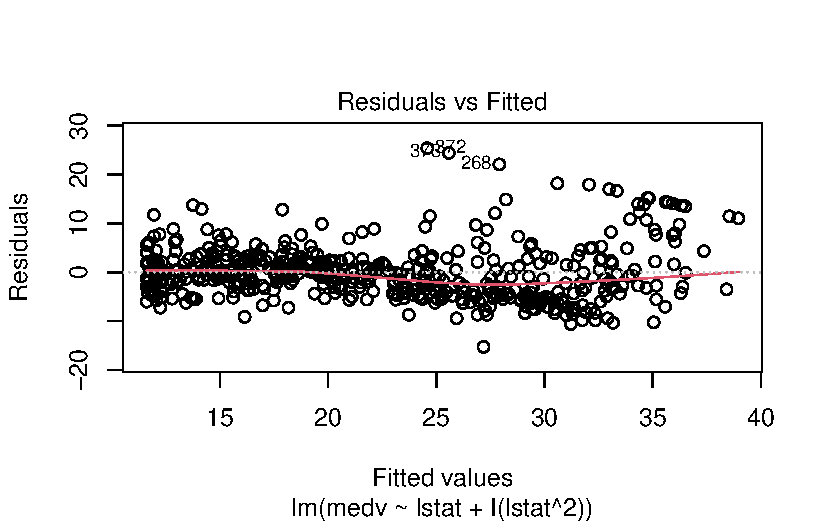
\includegraphics{Resumen-2---3_files/figure-pdf/unnamed-chunk-21-1.pdf}

}

\end{figure}

\begin{figure}[H]

{\centering 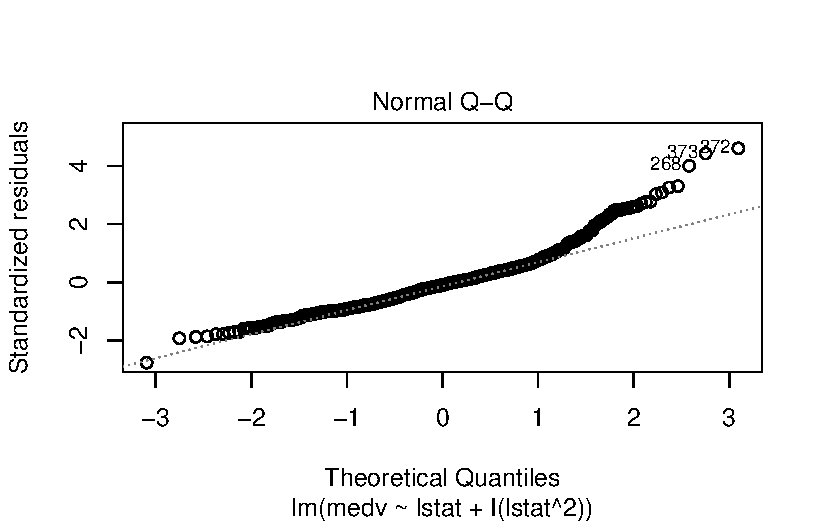
\includegraphics{Resumen-2---3_files/figure-pdf/unnamed-chunk-21-2.pdf}

}

\end{figure}

\begin{figure}[H]

{\centering 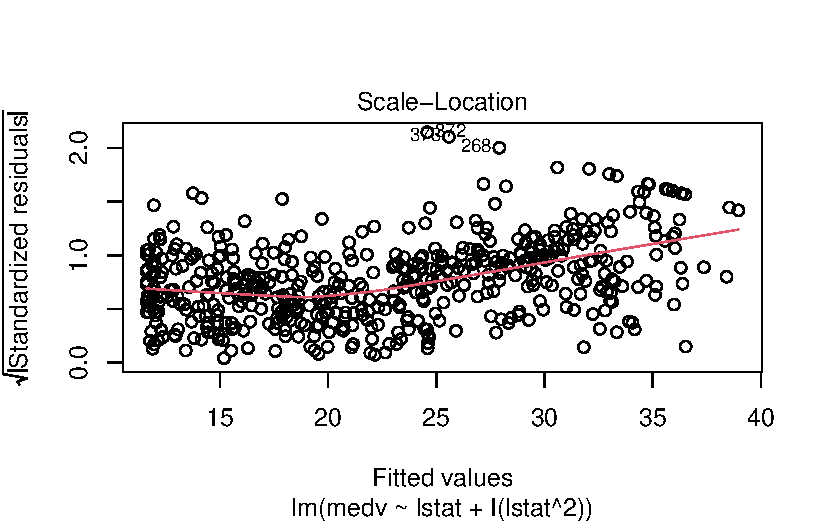
\includegraphics{Resumen-2---3_files/figure-pdf/unnamed-chunk-21-3.pdf}

}

\end{figure}

\begin{figure}[H]

{\centering 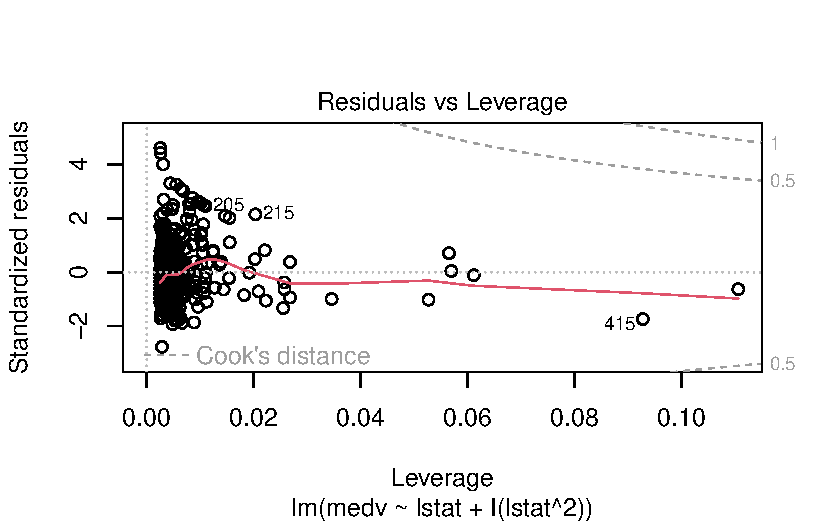
\includegraphics{Resumen-2---3_files/figure-pdf/unnamed-chunk-21-4.pdf}

}

\end{figure}

\begin{Shaded}
\begin{Highlighting}[]
\FunctionTok{par}\NormalTok{(}\AttributeTok{mfrow=}\FunctionTok{c}\NormalTok{(}\DecValTok{2}\NormalTok{,}\DecValTok{2}\NormalTok{))}
\end{Highlighting}
\end{Shaded}

Cuando se incluye lstat2 en el modelo se puede observar que hay pocos
patrones dicernibles en los residuos.

Par crear un ajuste mayor se puede utilizar la función \textbf{poly()}.

\begin{Shaded}
\begin{Highlighting}[]
\NormalTok{lm.fit5}\OtherTok{\textless{}{-}}\FunctionTok{lm}\NormalTok{(medv}\SpecialCharTok{\textasciitilde{}}\FunctionTok{poly}\NormalTok{(lstat,}\DecValTok{5}\NormalTok{))}
\FunctionTok{summary}\NormalTok{(lm.fit5)}
\end{Highlighting}
\end{Shaded}

\begin{verbatim}

Call:
lm(formula = medv ~ poly(lstat, 5))

Residuals:
     Min       1Q   Median       3Q      Max 
-13.5433  -3.1039  -0.7052   2.0844  27.1153 

Coefficients:
                 Estimate Std. Error t value Pr(>|t|)    
(Intercept)       22.5328     0.2318  97.197  < 2e-16 ***
poly(lstat, 5)1 -152.4595     5.2148 -29.236  < 2e-16 ***
poly(lstat, 5)2   64.2272     5.2148  12.316  < 2e-16 ***
poly(lstat, 5)3  -27.0511     5.2148  -5.187 3.10e-07 ***
poly(lstat, 5)4   25.4517     5.2148   4.881 1.42e-06 ***
poly(lstat, 5)5  -19.2524     5.2148  -3.692 0.000247 ***
---
Signif. codes:  0 '***' 0.001 '**' 0.01 '*' 0.05 '.' 0.1 ' ' 1

Residual standard error: 5.215 on 500 degrees of freedom
Multiple R-squared:  0.6817,    Adjusted R-squared:  0.6785 
F-statistic: 214.2 on 5 and 500 DF,  p-value: < 2.2e-16
\end{verbatim}

Incluir términos de hasta quinto orden mejora el ajuste del modelo, pero
si son mayores a este orden el modelo no tendrá valores p significativos
en el ajuste de regresión.

Para obtener los polinomios brutos de la función poly(), debe utilizarse
el argumento raw = TRUE.

\textbf{Tranformación logarítmica:}

\begin{Shaded}
\begin{Highlighting}[]
\FunctionTok{summary}\NormalTok{(}\FunctionTok{lm}\NormalTok{(medv}\SpecialCharTok{\textasciitilde{}}\FunctionTok{log}\NormalTok{(rm),}\AttributeTok{data =}\NormalTok{ Boston))}
\end{Highlighting}
\end{Shaded}

\begin{verbatim}

Call:
lm(formula = medv ~ log(rm), data = Boston)

Residuals:
    Min      1Q  Median      3Q     Max 
-19.487  -2.875  -0.104   2.837  39.816 

Coefficients:
            Estimate Std. Error t value Pr(>|t|)    
(Intercept)  -76.488      5.028  -15.21   <2e-16 ***
log(rm)       54.055      2.739   19.73   <2e-16 ***
---
Signif. codes:  0 '***' 0.001 '**' 0.01 '*' 0.05 '.' 0.1 ' ' 1

Residual standard error: 6.915 on 504 degrees of freedom
Multiple R-squared:  0.4358,    Adjusted R-squared:  0.4347 
F-statistic: 389.3 on 1 and 504 DF,  p-value: < 2.2e-16
\end{verbatim}

\hypertarget{predictores-cualitativos-1}{%
\subsection{Predictores cualitativos}\label{predictores-cualitativos-1}}

Para esta parte se usará: Carseats data para intentar predecir las
ventas de asientos de autos en 4000 localidades basado en una serie de
predictores.

\begin{Shaded}
\begin{Highlighting}[]
\FunctionTok{head}\NormalTok{(Carseats)}
\end{Highlighting}
\end{Shaded}

\begin{verbatim}
  Sales CompPrice Income Advertising Population Price ShelveLoc Age Education
1  9.50       138     73          11        276   120       Bad  42        17
2 11.22       111     48          16        260    83      Good  65        10
3 10.06       113     35          10        269    80    Medium  59        12
4  7.40       117    100           4        466    97    Medium  55        14
5  4.15       141     64           3        340   128       Bad  38        13
6 10.81       124    113          13        501    72       Bad  78        16
  Urban  US
1   Yes Yes
2   Yes Yes
3   Yes Yes
4   Yes Yes
5   Yes  No
6    No Yes
\end{verbatim}

Predictores cualitativos incluidos: Shelveloc (calidad de la ubicación
de la estantería). Tiene 3 valores posibles: Malo, medio y bueno. A
continuación ajustamos un modelo de regresión múltiple que incluye
algunos términos de interacción.

\begin{Shaded}
\begin{Highlighting}[]
\NormalTok{lm.fit}\OtherTok{\textless{}{-}}\FunctionTok{lm}\NormalTok{(Sales}\SpecialCharTok{\textasciitilde{}}\NormalTok{.}\SpecialCharTok{+}\NormalTok{Income}\SpecialCharTok{:}\NormalTok{Advertising}\SpecialCharTok{+}\NormalTok{Price}\SpecialCharTok{:}\NormalTok{Age,}\AttributeTok{data =}\NormalTok{ Carseats)}
\FunctionTok{summary}\NormalTok{(lm.fit)}
\end{Highlighting}
\end{Shaded}

\begin{verbatim}

Call:
lm(formula = Sales ~ . + Income:Advertising + Price:Age, data = Carseats)

Residuals:
    Min      1Q  Median      3Q     Max 
-2.9208 -0.7503  0.0177  0.6754  3.3413 

Coefficients:
                     Estimate Std. Error t value Pr(>|t|)    
(Intercept)         6.5755654  1.0087470   6.519 2.22e-10 ***
CompPrice           0.0929371  0.0041183  22.567  < 2e-16 ***
Income              0.0108940  0.0026044   4.183 3.57e-05 ***
Advertising         0.0702462  0.0226091   3.107 0.002030 ** 
Population          0.0001592  0.0003679   0.433 0.665330    
Price              -0.1008064  0.0074399 -13.549  < 2e-16 ***
ShelveLocGood       4.8486762  0.1528378  31.724  < 2e-16 ***
ShelveLocMedium     1.9532620  0.1257682  15.531  < 2e-16 ***
Age                -0.0579466  0.0159506  -3.633 0.000318 ***
Education          -0.0208525  0.0196131  -1.063 0.288361    
UrbanYes            0.1401597  0.1124019   1.247 0.213171    
USYes              -0.1575571  0.1489234  -1.058 0.290729    
Income:Advertising  0.0007510  0.0002784   2.698 0.007290 ** 
Price:Age           0.0001068  0.0001333   0.801 0.423812    
---
Signif. codes:  0 '***' 0.001 '**' 0.01 '*' 0.05 '.' 0.1 ' ' 1

Residual standard error: 1.011 on 386 degrees of freedom
Multiple R-squared:  0.8761,    Adjusted R-squared:  0.8719 
F-statistic:   210 on 13 and 386 DF,  p-value: < 2.2e-16
\end{verbatim}

contrasts() devuelve la codificación que R utiliza para las variables
ficticias.

\begin{Shaded}
\begin{Highlighting}[]
\FunctionTok{attach}\NormalTok{(Carseats)}
\FunctionTok{contrasts}\NormalTok{(ShelveLoc)}
\end{Highlighting}
\end{Shaded}

\begin{verbatim}
       Good Medium
Bad       0      0
Good      1      0
Medium    0      1
\end{verbatim}

ShelveLocGood que toma un valor de 1 si la ubicación de la estantería es
buena, y 0 en caso contrario.

El hecho de que el coeficiente de ShelveLocGood en el resultado de la
regresión sea positivo indica que una buena estanterías se asocia a
ventas elevadas (en comparación con las malas).

ShelveLocMedium tiene un coeficiente positivo menor, lo que indica tiene
ubicación media de las estanterías se asocia a mayores ventas que a una
mala ubicación, pero con menores ventas que una buena ubicación.

\hypertarget{funciones-de-escritura}{%
\subsection{Funciones de escritura}\label{funciones-de-escritura}}

\begin{Shaded}
\begin{Highlighting}[]
\NormalTok{LoadLibraries }\OtherTok{\textless{}{-}} \ControlFlowTok{function}\NormalTok{ () \{}
\FunctionTok{library}\NormalTok{ (ISLR2)}
\FunctionTok{library}\NormalTok{ (MASS)}
\FunctionTok{print}\NormalTok{ (}\StringTok{"The libraries have been loaded ."}\NormalTok{)}
\NormalTok{\}}
\end{Highlighting}
\end{Shaded}

Ahora si se escribe LoadLibraries, R dirá qué contiene la función.

\begin{Shaded}
\begin{Highlighting}[]
\NormalTok{LoadLibraries}
\end{Highlighting}
\end{Shaded}

\begin{verbatim}
function () {
library (ISLR2)
library (MASS)
print ("The libraries have been loaded .")
}
\end{verbatim}

Si llamamos a la función, las librerías se cargan y la sentencia print
se imprime.

\begin{Shaded}
\begin{Highlighting}[]
\FunctionTok{LoadLibraries}\NormalTok{()}
\end{Highlighting}
\end{Shaded}

\begin{verbatim}
[1] "The libraries have been loaded ."
\end{verbatim}



\end{document}
